\documentclass[9pt]{beamer}

%%pacotes referentes ao Beamer
%\useoutertheme{split}
%\setbeamertemplate{navigation symbols}{}

%\usetheme{beamertheme}
%\usebeamercolor{beamer-color name}

%\usetheme{Boadilla}
%\usecolortheme{dove}

\usetheme{CambridgeUS}
\usecolortheme{beaver}

% \usetheme{pittsburgh}
% \usecolortheme{dolphin}
%\usecolortheme{dove}
%\usecolortheme{seahorse}

%\usetheme{Montpellier}

%number in figures an tables -- beamer
\setbeamertemplate{caption}[numbered]

%Colocar no description
%[leftmargin=!,labelwidth=\widthof{Turma A}]
	
%pacotes usuais do latex
\usepackage[portuguese]{babel}
\usepackage[utf8]{inputenc}
\usepackage{bm}
\usepackage{graphicx}
%\usepackage{subfigure}
\usepackage[round]{natbib}
\usepackage{tikz}
\usetikzlibrary{shapes,arrows}
\usepackage{natbib}
\usepackage{times}
\usepackage{calc} %computes the length of a string
\usepackage{dsfont} %pacote para o 1 estilisado para indicadora
\usepackage{enumerate} %permite fazer uns enumerates diferentes
\usepackage[font=small,labelfont=bf]{caption} %permite colocar um segundo caption
\usepackage{subcaption}
\usepackage{booktabs} % comando \toprule, \midrule e \bottomrule
\usepackage{times} %times new roman font
\usepackage{multirow} %comando \multirow
\usepackage{setspace}
\usepackage{xcolor} %texto colorido
\usepackage{booktabs} %costumized tabs


%código para alinhar a esquerda os itens no description
\defbeamertemplate{description item}{align left}{\insertdescriptionitem\hfill}
\defbeamertemplate{enumerate item}{align left}{\insertdescriptionitem\hfill}



%AMS packages
\usepackage{amsmath}
\usepackage{amsfonts}
\usepackage{amssymb}

%Não quebre linhas
\binoppenalty=\maxdimen
\relpenalty=\maxdimen

%Comandos criados por mim
\DeclareMathOperator*{\argmin}{arg\,min}

\DeclareMathOperator*{\argmax}{arg\,max}


\DeclareMathOperator{\espe}{E}

\DeclareMathOperator{\spann}{span}

\DeclareMathOperator{\cov}{Cov}

\DeclareMathOperator{\vari}{Var}

%Informações para o primeiro slide
\date{}
\title[Probabilidade]{Variável aleatória contínua}
\author[Gilberto Sassi]{Gilberto Pereira Sassi}
\institute[IME -- UFBA]{Universidade Federal da Bahia \\ Instituto de Matem\'{a}tica e Estat\'{i}stica\\ Departamento de Estat\'{i}stica }

\begin{document}
	
\tikzstyle{decision} = [diamond, draw, fill=blue!20, 
text width=4.5em, text badly centered, node distance=3cm, inner sep=0pt]
\tikzstyle{block} = [rectangle, draw, fill=blue!20, 
text width=5em, text centered, rounded corners, minimum height=4em]
\tikzstyle{line} = [draw, -latex]
\tikzstyle{cloud} = [draw, ellipse,fill=red!20, node distance=3cm,
minimum height=2em]
	
\begin{frame}{}
	\maketitle
\end{frame}

\section{Motivação}

%slide 1
\begin{frame}{}

{\small
 \begin{block}{Objetivo}
  Caracterização probabilística de variáveis quantitativas contínuas. Neste caso, não existe interesse interesse em atribuir probabilidades a cada valor individual
  da variável e estamos interessados em atribuir probabilidades para intervalos da variável.
 \end{block}
% 
% \begin{block}{Exemplo de motivação}
%  Considere um círculo, com medidas de ângulos em graus, a partir de uma determinada origem. Neste círculo, tem um ponteiro que é colocado para girar no sentido anti-horário, conforme ilustrado pela figura.
% 
% 
% \begin{figure}[ht]
%  \centering
%  \caption{}
%  \begin{tikzpicture}[scale=0.9]
%   \draw[->] (-1,0) -- (1,0);
%   \draw[->] (0,-1) -- (0,1);
%   \draw[->] (0,0) -- (0.49, 0.49);
%   \draw (0,0) circle (0.7cm);
%   \draw[->]  (0.25, 0) arc (0:45:0.25cm);
%   \node [right] at (1,0) {\tiny $0^\circ$};
%   \node [above] at (0, 1) {\tiny $90^\circ$};
%   \node [left] at (-1, 0) {\tiny $180^\circ$};
%   \node [below] at (0,-1) {\tiny $270^\circ$};
%   \node [above right] at (0.22, 0) {\tiny $x$};
%  \end{tikzpicture}
% \end{figure}
%  
%  
%  Seja $X$ a variável que indicar o ponto em que o ponteiro para. Assuma que não existe razão de preferência para onde o ponteiro pode parar.
% \end{block}

Para uma variável quantitativa contínua $X$, podemos construir o histograma que é válido para uma amostra específica. Para uma outra amostra da variável quantitativa contínua X na mesma população, podemos obter um histograma ligeiramente diferente. A ideia é obter uma curva ou uma função que aproxime bem o formato de todos histogramas, conforme ilustrado na figura. Chamamos esta curva de \textcolor{blue}{função densidade de probabilidade} ou simplesmente \textcolor{blue}{função densidade}. 
\begin{figure}[htbp]
	\centering
	\caption{Histogramas sobrepostos para diversas amostras da variável $X$. A linha azul é a função densidade de probabilidade da variável quantitativa contínua $X$.}
	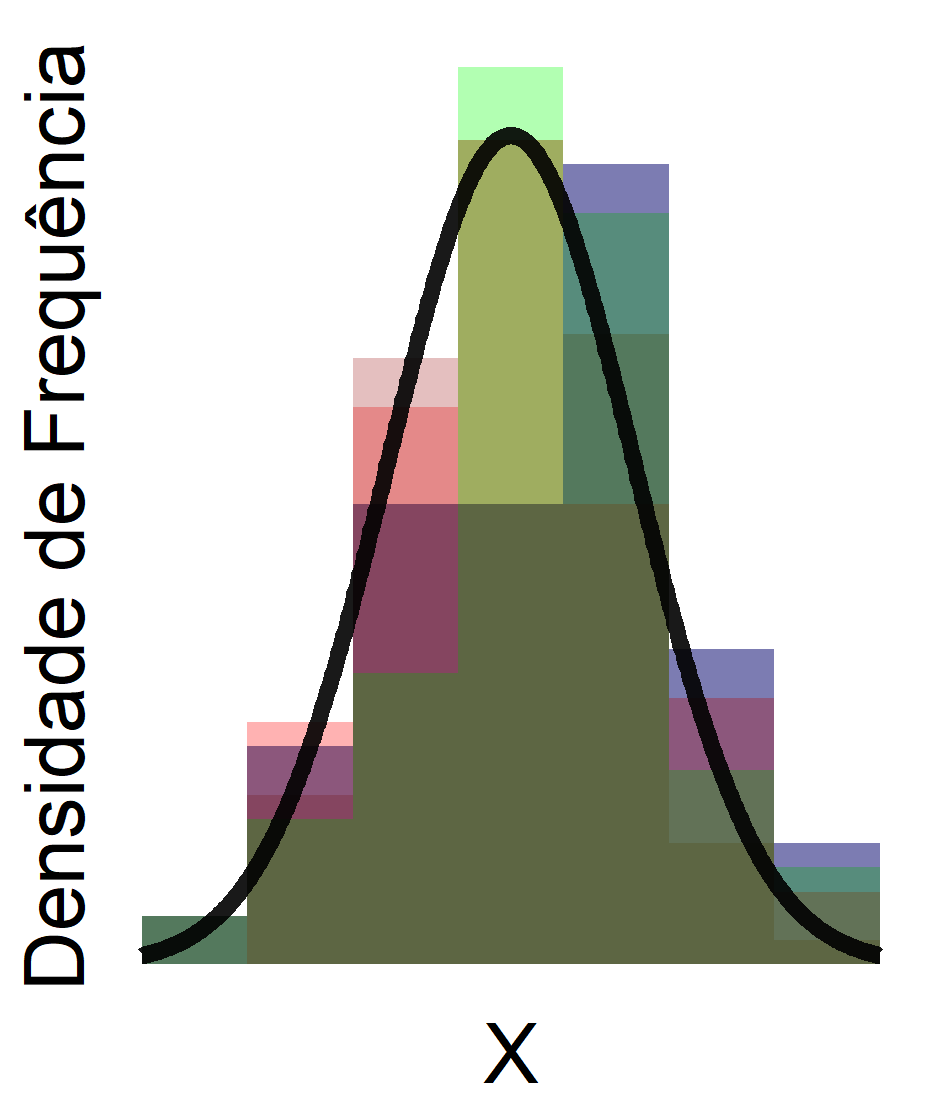
\includegraphics[width=3cm]{figure/motivacao.png}
\end{figure}
}
\end{frame}

% %slide 2
% \begin{frame}{Exemplo de motivação}
%  Considere um círculo, com medidas de ângulos em graus, a partir de uma determinada origem. Neste círculo, tem um ponteiro que é colocado para girar no sentido anti-horário, conforme ilustrado pela figura.
%  
%  {\scriptsize
%  \begin{figure}[ht]
%   \centering
%   \caption{}
%   \begin{tikzpicture}
%    \draw[->] (-1,0) -- (1,0);
%    \draw[->] (0,-1) -- (0,1);
%    \draw (0,0) -- (0.49, 0.49);
%    \draw (0,0) circle (0.7cm);
%    \draw [->] (0.25, 0) arc (0:45:0.25cm);
%    \node [right] at (1,0) {$0^\circ$};
%    \node [above] at (0, 1) {$90^\circ$};
%    \node [left] at (-1, 0) {$180^\circ$};
%    \node [below] at (0,-1) {$270^\circ$};
%    \node [above right] at (0.22, 0) {$x$};
%   \end{tikzpicture}
%  \end{figure}
%   }
%   
%   Seja $X$ a variável que indicar o ponto em que o ponteiro para. Assuma que não existe razão de preferência para onde o ponteiro pode parar.
% \end{frame}


%\begin{frame}{Exemplo de motivação -- continuação}
% 
% Então a probabilidade dos intervalos $(x, x+\Delta]$ é $\dfrac{\Delta}{360}$ e podemos construir um gráfico semelhante ao histograma.
% 
% {\footnotesize
% \begin{figure}[ht]
%  \centering
%  \caption{}
%  \begin{tikzpicture}
%   \draw [->] (0,0) -- (6,0);
%   \draw [->] (0,0) -- (0,1);
%   \draw [dotted] (0,0.5) -- (5,0.5);
%   \draw [dotted] (1,0) -- (1,0.5);
%   \draw [dotted] (2,0) -- (2,0.5);
%   \draw [dotted] (4,0) -- (4,0.5);
%   \draw [dotted] (5,0) -- (5,0.5);
%   \node [right] at (6,0) {$x$};
%   \node [above] at (0,1) {$f(x)$};
%   \node [left] at (0,0.5) {$\frac{1}{360}$};
%   \node [below] at (1,0) {$\Delta$};
%   \node [below] at (2,0) {$2\Delta$};
%   \node [below] at (3,0) {$\cdots$};
%   \node [below] at (4,0) {$360-\Delta$};
%   \node [below] at (5,0) {$360$};
%  \end{tikzpicture}
% \end{figure}
% }
% 
% Ao fazermos $\Delta$ pequeno, podemos usar este gráfico para qualquer intervalo $(a,b)$.
% 
% {\footnotesize
% \begin{figure}[ht]
%  \centering
%  \caption{}
%  \begin{tikzpicture}
%   \draw [->] (0,0) -- (6,0);
%   \draw [->] (0,0) -- (0,1);
%   \draw [dotted] (1,0.5) -- (3,0.5);
%   \draw [dotted] (1,0) -- (1,0.5);
%   \draw [dotted] (3,0) -- (3,0.5);
%   \node [right] at (6,0) {$x$};
%   \node [above] at (0,1) {$f(x)$};
%   \node [left] at (0,0.5) {$\frac{1}{360}$};
%   \node [below] at (1,0) {$a$};
%   \node [below] at (3,0) {$b$};
%   \draw [dotted, fill = gray!40] (1,0) rectangle (3,0.5);
%  \end{tikzpicture}
% \end{figure}
% }
% 
%\end{frame}

\section{Definição}
\begin{frame}{Definição}

{\scriptsize
\begin{block}{Modelo de probabilidade}
	Um modelo probabilidade para uma variável quantitativa contínua $X$ é estabelecido quando definimos:
	\begin{enumerate}[i.]
		\item os valores possíveis para a variável quantitativa contínua;
		\item a função densidade de probabilidade. 
	\end{enumerate}
	Quando temos uma função densidade de probabilidade associada a uma variável $X$, dizemos que $X$ é uma \textcolor{blue}{variável aleatória contínua} para deixar claro que temos um modelo de probabilidade para $X$.
\end{block}
\vfill

\begin{block}{Definição}
 Dizemos que $f(x)$ é uma função densidade de probabilidade para um variável aleatória contínua $X$ se satisfaz duas condições:
 \begin{enumerate}[i.]
  \item $f(x) \geq 0$;
  \item A área delimitada por $f(x)$ e o eixo x é igual a 1.
 \end{enumerate} 
\end{block}
\vfill

\begin{block}{Observação}
 \begin{enumerate}[1)]
  \item Note que $P(X=x)=0,$ para $x\in [a,b]$, logo $P(a < X \leq b) = P(a < X <b) = P(a \leq X <b) = P(a \leq X \leq b)$.
  \item A área sob a curva da função densidade de probabilidade é igual a $P(a < X < b)$ como ilustrado na figura~\ref{fig:area_prob}.
 \end{enumerate}
\end{block}
}
\end{frame}

\begin{frame}{Área sob a curva como probabilidade.}
\begin{figure}
	\centering
	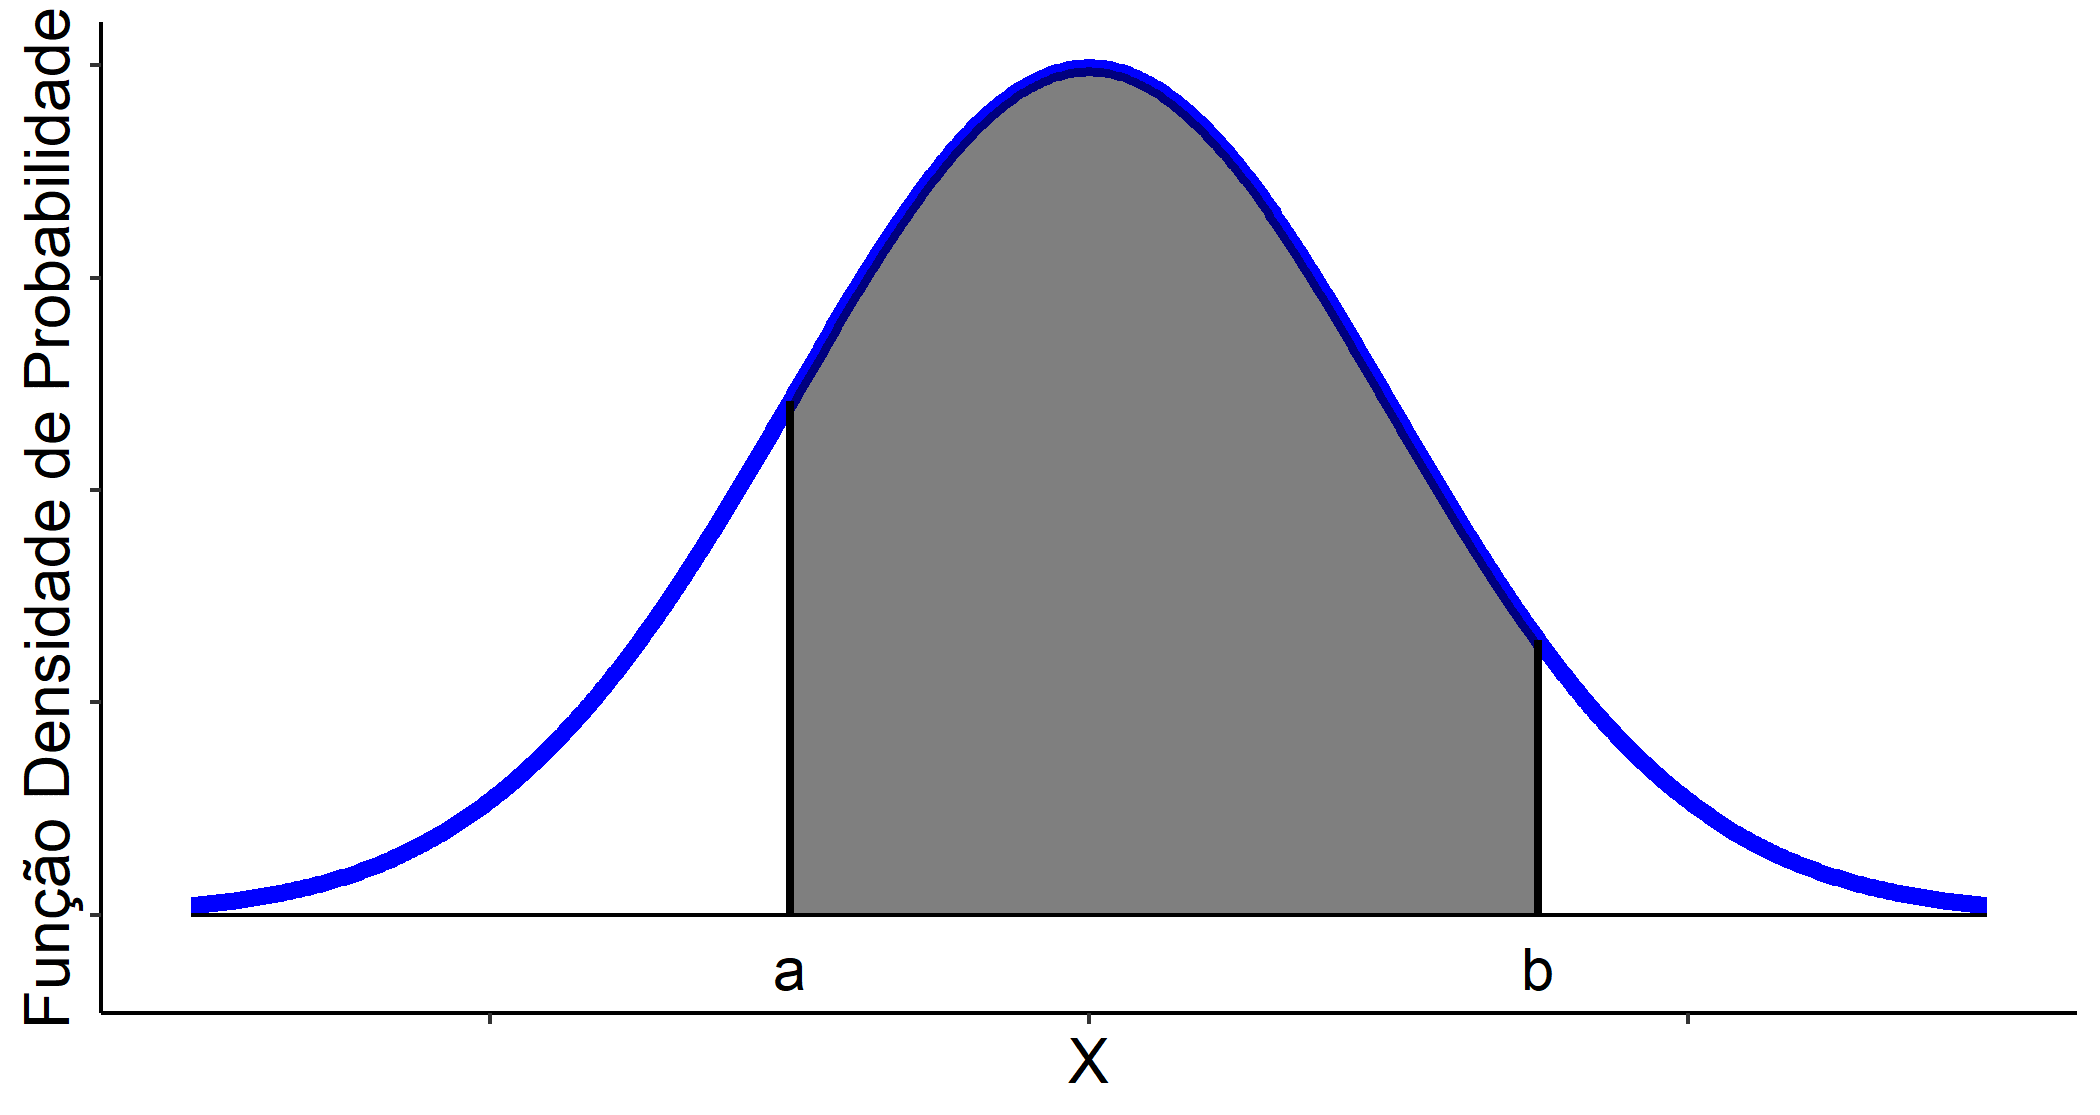
\includegraphics[width=12cm]{figure/probabilidade.png}
	\caption{Probabilidade de uma variável aleatória contínua $X$ estar entre $a$ e $b$. A área pintada no gráfico é o valor de $P(a < X < b)$.}
	\label{fig:area_prob}
\end{figure}

\end{frame}

\begin{frame}{Exemplo}
 Num teste tradicional com crianças, o tempo em minutos para a realização de uma bateria de questões de raciocínio verbal e lógico é uma variável aleatória contínua $T$ com função densidade de probabilidade
 dada por
 \begin{align*}
  f(t) =
  \begin{cases}
   \dfrac{t-4}{40}, & \mbox{ se } 8 \leq t < 10,\\
   \dfrac{3}{20}, & \mbox{ se } 10 \leq t \leq 15,\\
   0, & \mbox{ caso contrário}.
  \end{cases}
 \end{align*}
  Qual a probabilidade de uma criança responder a bateria de teste entre 9 e 12 minutos?
\end{frame}

\begin{frame}{Exemplo}
$P(9 < X \leq 12)$ é  área delimitada pelo gráfico conforme figura~\ref{fig:exemplo}.

{\tiny
\begin{figure}[ht]
\centering
\caption{Função denside.}
\label{fig:exemplo}
 \begin{tikzpicture}
     \draw [->] (0,0) -- (10,0);
     \draw [thick] (0,0) -- (4,0);
     \draw (4,0) circle (0.05cm);
     \draw [thick] (7.5,0) -- (10,0);
     \draw (7.5,0) circle (0.05cm);
     \draw [thick] (4, 0.5) -- (5, 0.75);
     \draw [fill] (4, 0.5) circle (0.05cm);
     \draw [->] (0,0) -- (0,1);
     \draw [thick] (5, 0.75) -- (7.5, 0.75);
     \draw [fill] (7.5, 0.75) circle (0.05cm);
     \node [left] at (0, 0.5) {$0.1$};
     \node [left] at (0, 0.75) {$0.15$};
     \draw [fill] (0, 0.5) circle (0.02cm);
     \draw [fill] (0, 0.75) circle (0.02cm);
     \draw [fill = gray!40, dotted] (4.5, 0) --  (5, 0) -- (5, 0.75) -- (4.5, 0.625) -- (4.5, 0);
     \draw [fill = gray!40, dotted] (5,0) rectangle (6,0.75);
     \node [below] at (4,0) {$8$};
     \node [below] at (4.5,0) {$9$};
     \node [below] at (5,0) {$10$};
     \node [below] at (6,0) {$12$};
     \node [below] at (7.5, 0) {$15$};
     \node [right, below] at (10, 0) {$x$};
     \node [above] at (0, 1) {$f(x)$};
     \node [below, left] at (0,0) {$(0,0)$};
 \end{tikzpicture}
\end{figure}
}

\begin{align*}
 P(9 < X \leq 12) &= 1 \cdot \dfrac{\frac{5}{40}+\frac{3}{20}}{2} + 2 \cdot \dfrac{3}{20}\\
 &= \dfrac{7}{16} \\
 &= 0,4375.
\end{align*}
\end{frame}

\section{Medidas de dispersão e e de posição: variáveis aleatórias contínuas}
\begin{frame}{Definição}
 \begin{itemize}
  \item Média: $\espe (X) = \mu = \int_{-\infty}^{\infty} x f(x) dx$;
  \vfill
  
  \item Mediana: valor $Md$ com a propriedade $P(X  \geq Md) \geq 0.5$ e $P(X \leq Md) \geq 0.5$;
  \vfill
  
  \item Moda: valor $Mo$ tal que $f(x) \leq f(Mo), \forall x$;
  \vfill
  
  \item Variância: $\vari (X) =  \sigma^2 = \int_{-\infty}^{\infty} (x-\mu)^2 f(x) dx$.
 \end{itemize}

\end{frame}

\section{Principais modelos para variáveis aleatórias contínuas}

\subsection{Modelo uniforme contínuo}

\begin{frame}{Modelo uniforme contínuo}
 Uma variável aleatória contínua $X$ tem distribuição uniforme contínua no intervalo $[a,b]$ se sua função densidade de probabilidade é dada por:
 \begin{align*}
  f(x) = \begin{cases}
          \dfrac{1}{b-a}, & \mbox{ se } a \leq x \leq b,\\
          0, & \mbox{ caso contrário }.
         \end{cases}
 \end{align*}
\begin{figure}[ht]
\centering
\caption{}
 \begin{tikzpicture}
     \draw [->] (0,0) -- (10,0);
     \draw [->] (0,0) -- (0,1);
     \draw [thick] (0,0) -- (4,0);
     \draw (4,0) circle (0.05cm);
     \draw [thick] (7,0) -- (10,0);
     \draw (7,0) circle (0.05cm);
     \draw [thick] (4,0.5) -- (7,0.5);
     \draw [fill] (4,0.5) circle (0.05cm);
     \draw [fill] (7, 0.5) circle (0.05cm);
     \node [below]  at (4,0) {$a$};
     \node [below] at (7, 0) {$b$};
     \node [left] at (0, 0.5) {$\frac{1}{b-a}$};
     \node [right] at (10, 0) {$x$};
     \node [above] at (0,1) {$f(x)$};
 \end{tikzpicture}
 \end{figure}
 \vfill
 
 \textbf{Notação:} $X \sim U[a, b]$.
 
% \begin{block}{Características numéricas}
%  Média: $\mu = \espe (x) = \dfrac{b+a}{2}$; Variância: $\sigma^2 = \vari (X) = \dfrac{(b-a)^2}{12}$; Mediana: $Md = \dfrac{b+a}{2}$.
% \end{block}
\end{frame}

\begin{frame}{Propriedades -- modelo uniforme contínuo}
\begin{enumerate}[i.]
 \item \textbf{Média} $\mu = \espe (x) = \dfrac{b+a}{2}$;
 \vfill
 
 \item \textbf{Variância:} $\sigma^2 = \vari (X) = \dfrac{(b-a)^2}{12}$;
 \vfill
 
 \item \textbf{Mediana:} $Md = \dfrac{b+a}{2}$;
 \vfill
 
 \item \textbf{Moda} $Mo:$ é qualquer número em $[a,b]$.
\end{enumerate}

\end{frame}


\begin{frame}{Exemplo}
 Admite-se que uma pane elétrica pode ocorrer em qualquer ponto de uma rede elétrica de 10km.
 \begin{enumerate}[a)]
  \item Qual a probabilidade da pane ocontecer nos primeiros 500 metros;
  \item O custo do reparo da rede depende da distância do centro do serviço ao local da pane. Considere que o centro de serviço está na origem da rede e que o custo é dado pela tabela
\begin{table}[ht]
\centering
\begin{tabular}{l|l}
  \toprule[0.025cm]
  Distância em km & Custo \\
  \midrule[0.025cm]
  $[0,3)$ & $R\$200,00$ \\ 
  $[3,8)$ & $R\$400,00$ \\ 
  $[8,10]$ & $R\$1000,00$ \\ 
   \toprule[0.025cm]
\end{tabular}
\end{table}
Qual o custo médio para reparar a rede?
 \end{enumerate}
\end{frame}

\begin{frame}{Solução:}
 A função de probabilidade é dada por
 
 {\tiny
 \begin{figure}[ht]
  \centering
  \caption{}
   \begin{tikzpicture}
     \draw [->] (-1,0) -- (11.2,0);
     \draw [->] (0,0) -- (0,1);
     \draw [thick] (-1,0) -- (0,0);
     \draw (0,0) circle (0.05cm);
     \draw [thick] (0,0.5) -- (10, 0.5);
     \draw [thick] (10,0) -- (11.2,0);
     \draw (10,0) circle (0.05cm);
     \draw [fill] (0,0.5) circle (0.05cm);
     \draw [fill] (10,0.5) circle (0.05cm);
     \node [right] at (11.2,0) {$x$};
     \node [above] at (0,1) {$f(x)$};
     \node [left] at (0,0.5) {$\dfrac{1}{10.000}$};
     \node [below] at (0,0) {$0$};
     \node [below] at (10,0) {$10.000$};
 \end{tikzpicture}
 \end{figure}
  }

  \begin{enumerate}[a)]
   \item $P(0 \leq X \leq 500) = \dfrac{500}{10.000} = \dfrac{1}{20} = 0,05$;
   \item \begin{itemize}
          \item $P(0 \leq X \leq 3.000) = \dfrac{3.000}{10.000} = 0,3$;
          \item $P(3.000 \leq X \leq 8.000) = \dfrac{5.000}{10.000} = \dfrac{1}{2} = 0,5$
          \item $P(8.000 \leq X) = \dfrac{2.000}{10.000} = \dfrac{1}{5} = 0,2$
         \end{itemize}
  \end{enumerate}

\end{frame}

\begin{frame}{Exemplo - continuação}
Ou seja, temos uma tabela de distância, custo e probabilidade dada por
\begin{table}[htbp]
\centering
\begin{tabular}{ccc}
  \toprule[0.025cm]
  Distância em km & Custo & Probabilidade de pane dentro da distância \\
  \midrule[0.025cm]
  $[0,3)$ & $R\$200,00$ & $0,3$ \\ 
  $[3,8)$ & $R\$400,00$ & $0,5$ \\ 
  $[8,10]$ & $R\$1000,00$ & $0,2$ \\ 
   \toprule[0.025cm]
\end{tabular}
\end{table}

 Então podemos estabelecer uma variável aleatória discreta $Y$, custo de reparo, com valores possíveis $200$, $400$ e $1000$ e função de probabilidade 
  \begin{align*}
  f(200) &= 0,3;\\
  f(400) &= 0,5;\\
  f(1000) &= 0,2.
  \end{align*}
  e o custo médio é dado por
  \begin{align*}
   \espe (Y) = 0,3 \cdot 200 + 0,5 \cdot 400 + 0,2 \cdot 1000 = 460.
  \end{align*}

  Ou seja, o custo médio de reparo para esta rede elétrica é de $R\$460,00$.
\end{frame}

\subsection{Modelo exponencial}

\begin{frame}{Modelo exponencial}
Uma variável aleatória contínua $X$ segue o modelo exponencial com parâmetro $\alpha$  se sua densidade é dada por
 $
  f(x) = \alpha e^{-\alpha \cdot x}
 $, para  $x  \geq 0$.
 
 \begin{figure}[ht]
  \centering
  \caption{}
  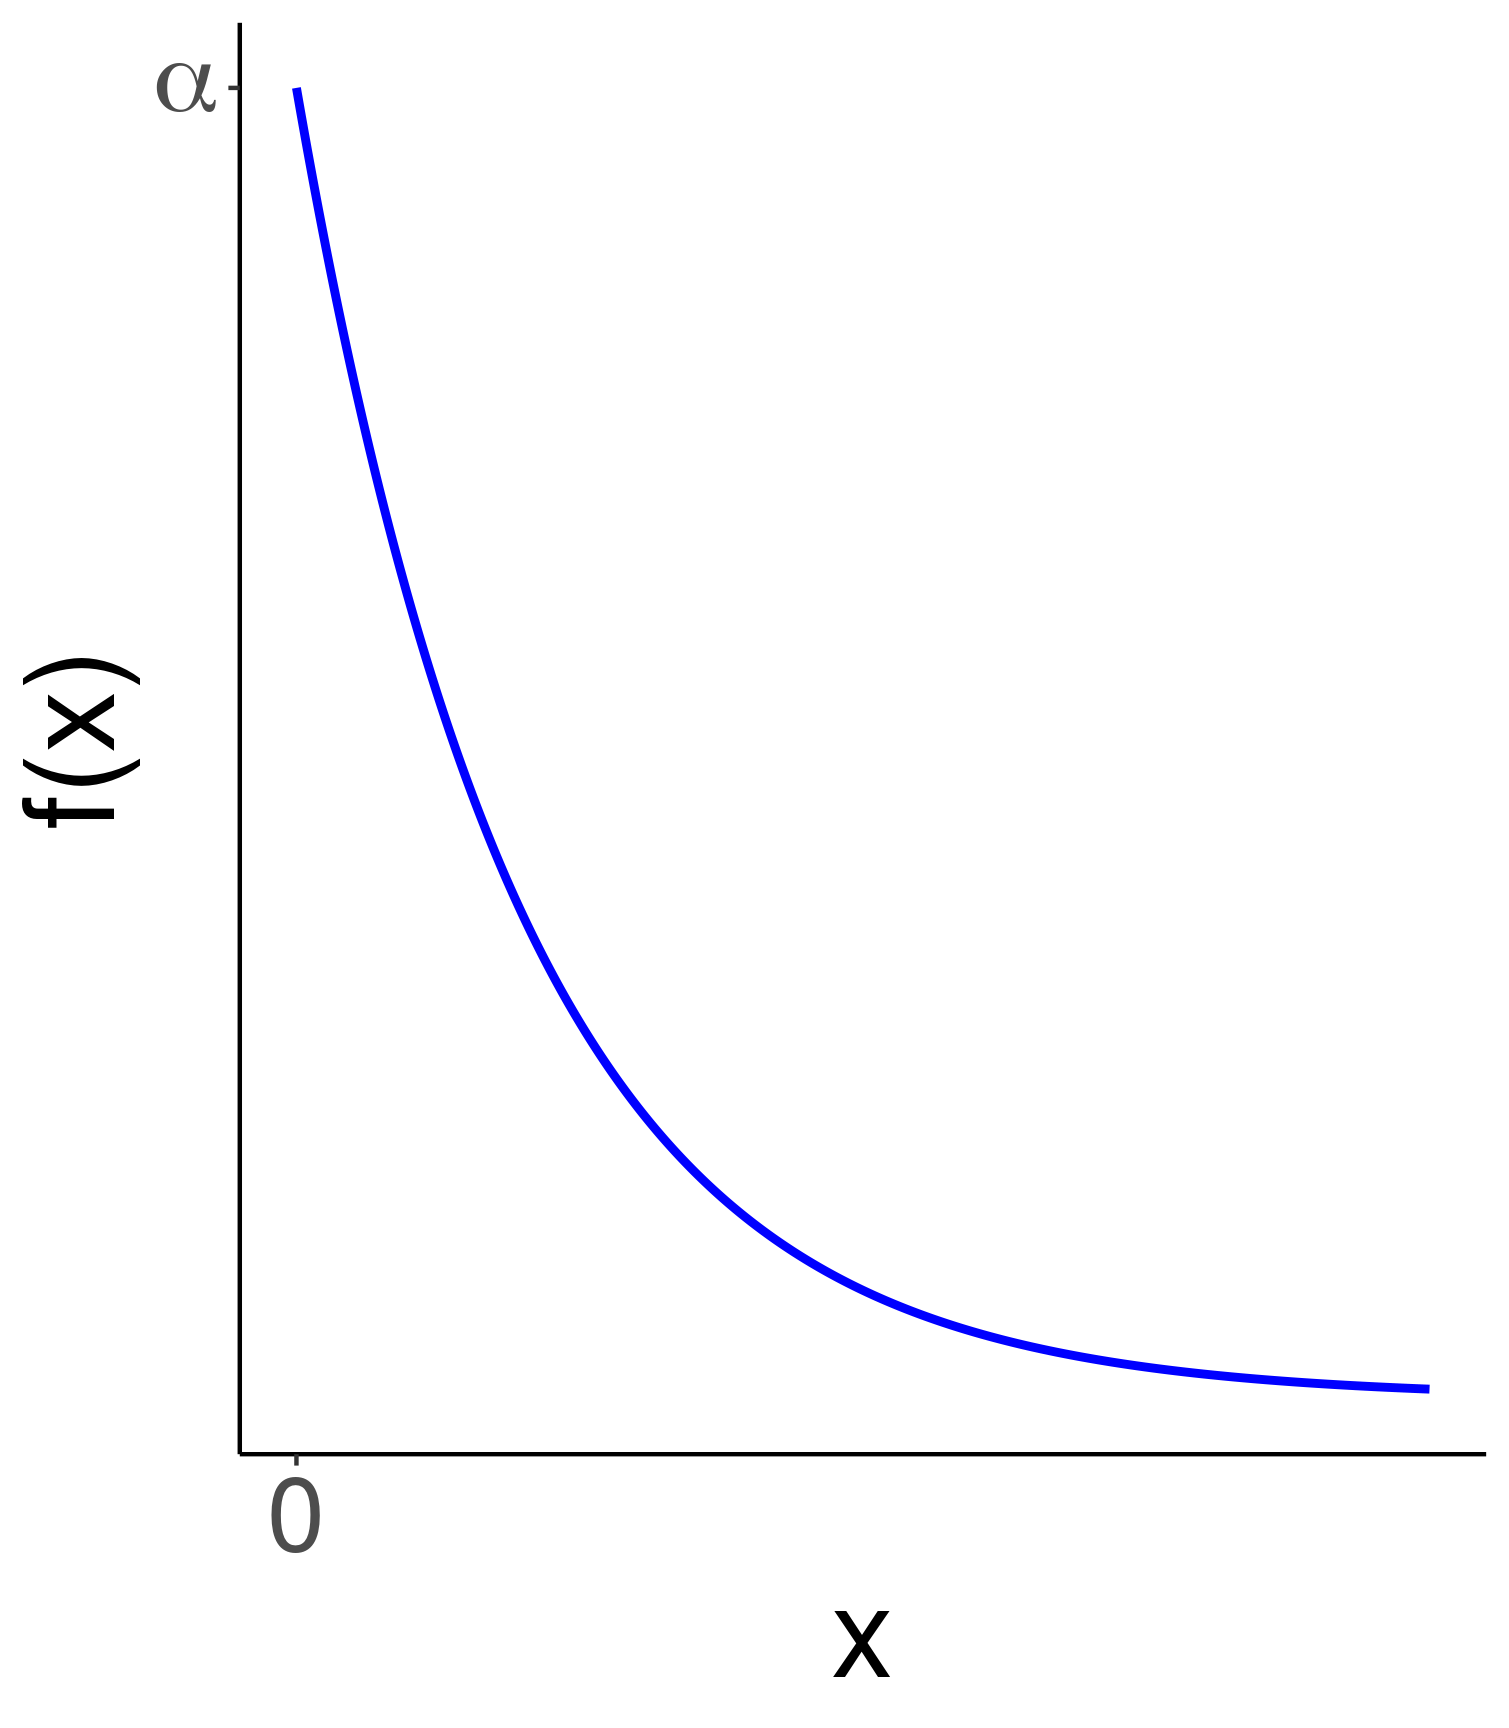
\includegraphics[width = 4cm]{figure/exp.png}
 \end{figure}
 \vfill
 
 \textbf{Notação:} $X \sim Exp(\alpha)$
 
%  \begin{block}{Características numéricas}
%   Média: $\espe(X) = \mu = \dfrac{1}{\alpha}$; Variância: $\sigma^2 = \dfrac{1}{\alpha^2}$;  Mediana: $Md = \dfrac{\log 2}{\alpha}$; Moda: $Mo = \alpha$.
%  \end{block}
\end{frame}

\begin{frame}{Propriedades -- modelo exponencial}
\begin{enumerate}[i.]
 \item \textbf{Média} $\espe(X) = \mu = \dfrac{1}{\alpha}$;
 \vfill
 
 \item \textbf{Variância:} $\vari(X) = \sigma^2 = \dfrac{1}{\alpha^2}$;
 \vfill
 
 \item \textbf{Mediana:} $Md(X) = \dfrac{\log 2}{\alpha}$;
 \vfill
 
 \item \textbf{Moda} $Mo = 0$.
\end{enumerate}

\end{frame}


\begin{frame}{Modelo exponencial}
 \begin{block}{Uso}
  Modelagem de tempo até ocorrer um exemplo. Por exemplo: tempo até o óbito, tempo até uma falha de um equipamento, tempo até solicitação ou ligação, etc.
 \end{block} 
\vfill
 
 \begin{block}{Cálculo da área sob a curva}
 Seja $X \sim Exp(\alpha)$, seja $a$ e $b$ com $a < b < \infty$ então
  \begin{itemize}
   \item Se $a > 0$, então $\int_{a}^{b} \alpha e^{-\alpha \cdot x} dx = e^{-\alpha\cdot a} - e^{-\alpha\cdot b}$;
   \vfill
   
   \item Se $a \leq 0$, então $\int_{a}^{b} \alpha e^{-\alpha \cdot x} dx = 1 - e^{-\alpha\cdot b}$.
  \end{itemize}

 \end{block}

\end{frame}


\begin{frame}{Exemplo}
  Sabe-se que um paciente em estágio avançado de uma certa enfermidade vive em média apenas em 120 dias. Qual a probabilidade de um paciente morrer antes de 90 dias?
  \vfill
 
 \textbf{Solução:}
 Pelo enunciado do exercício, temos que $\espe(X) = \dfrac{1}{\alpha} =  120$, ou seja, $\alpha = \dfrac{1}{120} = 0,008$. Então,
 \begin{align*}
  P(X \leq 90) = 1 - \exp (-0,008 \cdot 90) = 0,53.
 \end{align*}
  ou seja,  probabilidade do paciente morrer antes de 90 dias é 53\%.
\end{frame}

\subsection{Modelo normal}

\begin{frame}{Modelo normal}
Dizemos que uma variável aleatória contínua $X$ tem distribuição normal com parâmetro $\mu$ e $\sigma^2$ se sua função densidade de probabilidade é dada por:
\begin{align*}
 f(x) = \dfrac{1}{\sqrt{2 \pi \sigma^2}} \exp \left\{ -\dfrac{(x-\mu)^2}{2\sigma^2}  \right\}, \quad x \in \mathbb{R}.
\end{align*}

\begin{figure}[ht]
 \centering
 \caption{}
 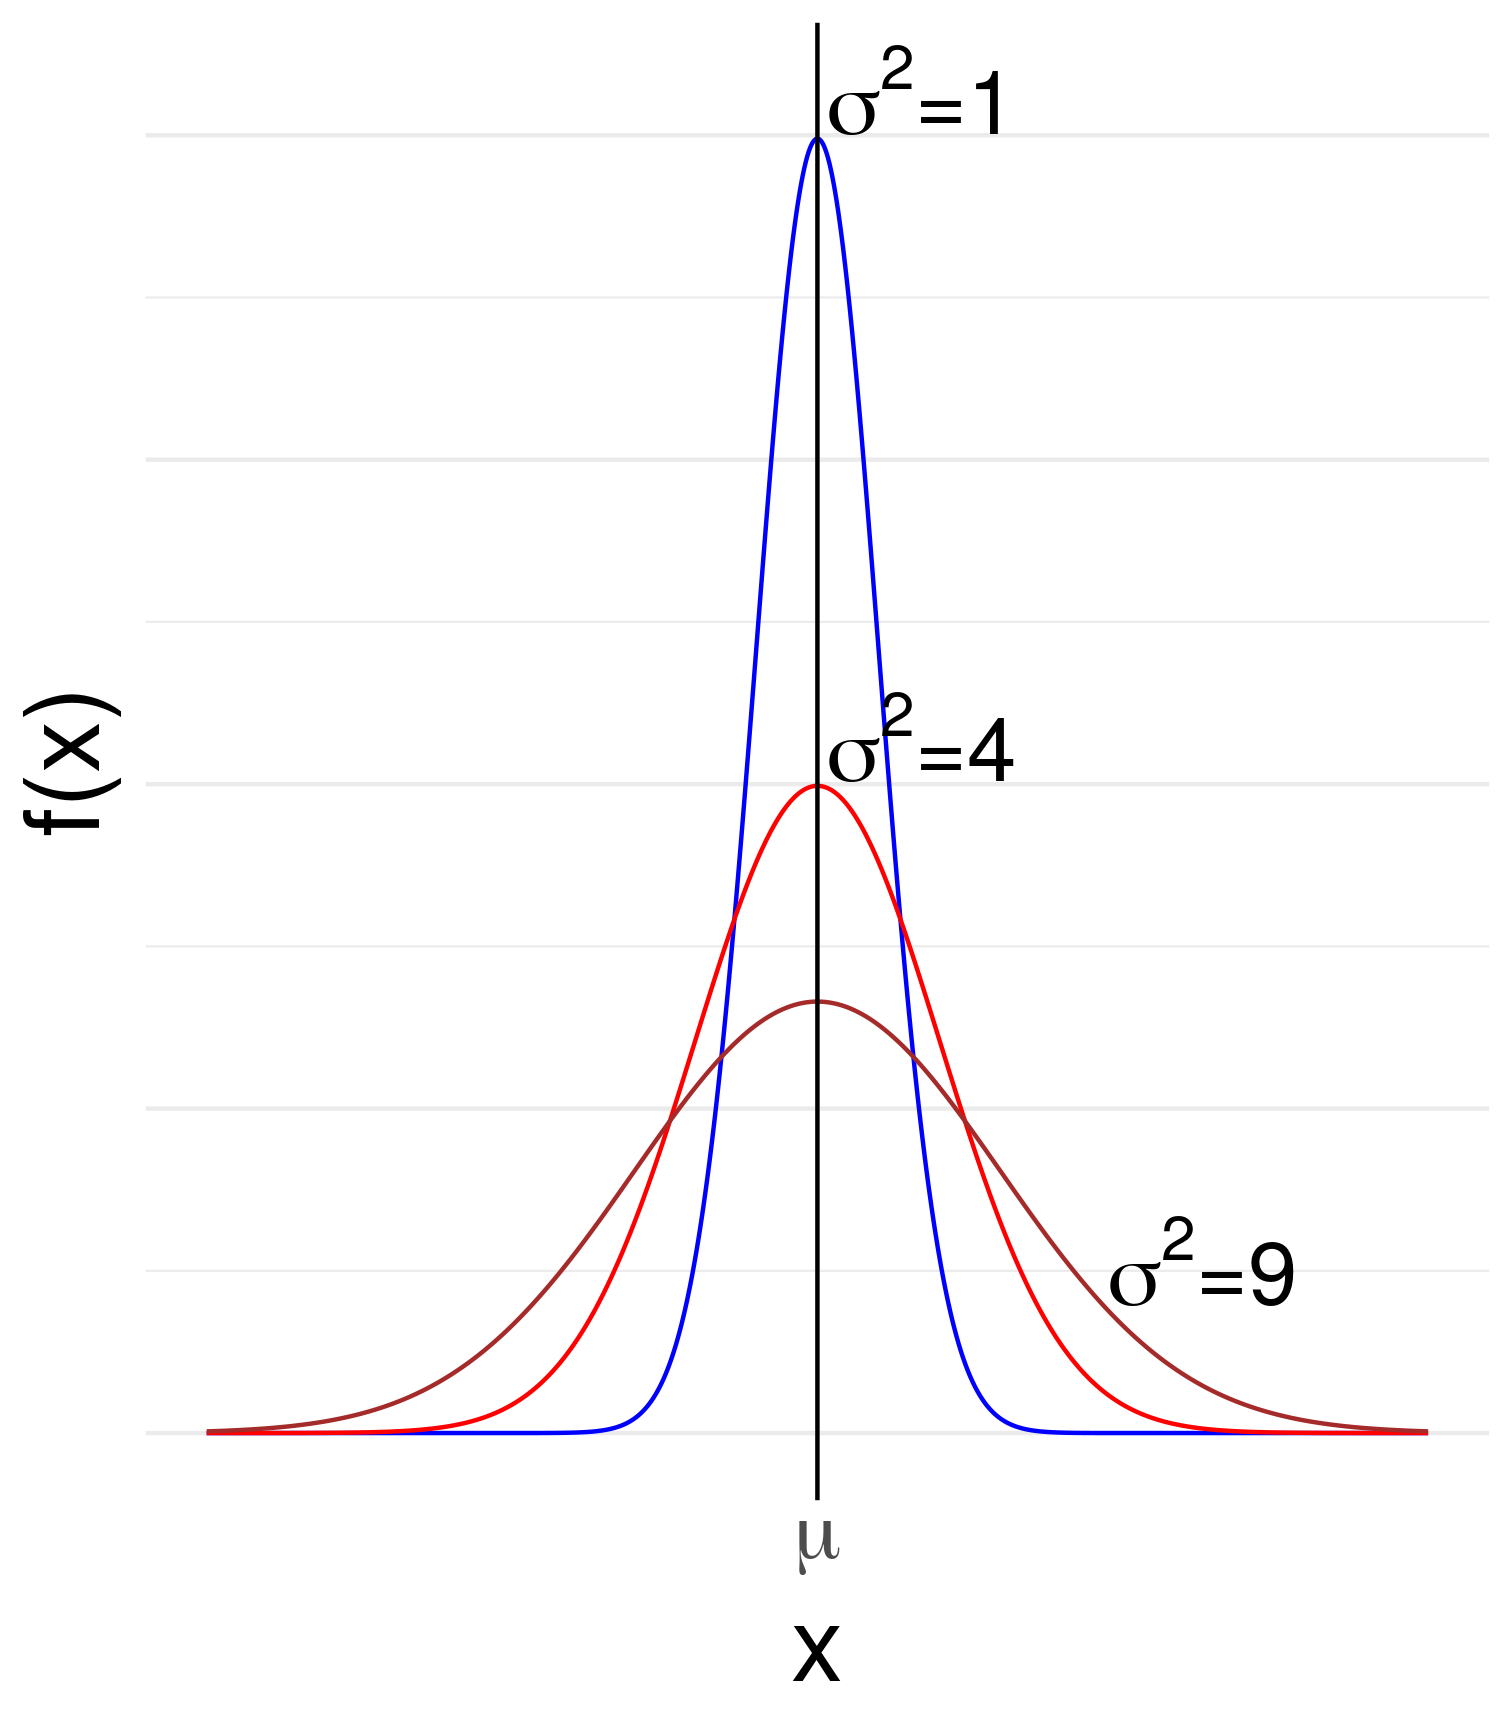
\includegraphics[height = 4.5cm]{figure/normal.png}
\end{figure}


\textbf{Notação:} $X \sim N(\mu, \sigma^2)$.

\end{frame}

\begin{frame}{Propriedade: modelo normal}
 \begin{enumerate}[i)]
 \item $f(x)$ é simétrica em relação a $\mu$;
 \vfill
 
 \item $f(x)$ tende a $0$ quando $x \rightarrow \pm \infty$;
 \vfill
 
 \item $\espe(X)= \mu$;
 \vfill
 
 \item $\vari(X) =\sigma^2$;
 \vfill
 
 \item A moda e a medianda de $X$ é $\mu$;
 \vfill
 
 \item \textcolor{red}{ $P(a < X \leq b) = P(a < X < b) = P(a \leq X < b) = P(a \leq X \leq b)$;}
 \vfill
 
 \item Se $-\infty \leq a < b \leq \infty$, então
 \begin{enumerate}[a)]
  \item \textcolor{red}{$P(a < X < b) = \Phi\left( \dfrac{b-\mu}{\sigma} \right) - \Phi\left( \dfrac{a-\mu}{\sigma} \right)$;}
  \item \textcolor{red}{$P(X < b) = \Phi\left( \dfrac{b-\mu}{\sigma} \right)$;}
 \end{enumerate}
 em que os valores de $\Phi(z)$ são tabelados;
 \vfill
 
 \item \textcolor{red}{ Se $c < 0$, então $\Phi(c) = 1 - \Phi(-c)$};
 \vfill
 
 \item Se $c= -\infty$, então $\Phi(c) = 0$;
 \vfill
 
 \item Se $c = \infty$, então $\Phi(c) = 1$.
\end{enumerate}
\end{frame}

\begin{frame}{Exemplo}
 Doentes, sofrendo de certa moléstia, são submetidos a um tratamento intensivo cujo tempo de cura foi modelado por uma densidade Normal de média 15 e desvio padrão 2. Qual a proporção desses pacientes
 demoram mais de 17 dias para se recuperar? Qual o tempo máximo para a recuperação de 25\% dos pacientes?
 
 \textbf{Solução:}
 Note que $X \sim N(15, 4)$.
 \begin{itemize}
  \item 
  \begin{align*}
  P(17 > X) &= 1 -  P(X \leq 17)\\
   &= 1 - \Phi\left( \dfrac{17-15}{\sqrt{4}} \right)\\
   &=\Phi(-1) = 0,1587.
  \end{align*}
  Ou seja, 16\% dos porcentagens pacientes demoram mais de 17 dias para se recuperar;
  \item $P(X \leq t) = \Phi\left( \dfrac{t-15}{2} \right) = 0,25$, então e $\dfrac{t-15}{2} = -0,68$ e $t = -0,68 \cdot 2 + 15 = 13,64$. Ou seja, o tempo máximo para recuperação de 25\% é de 2,651 dias.
 \end{itemize}
\end{frame}

\section{Aproximação Normal para o Modelo Binomial}

\begin{frame}{Aproximando a Função de Distribuição Acumada de $X \sim b(n; p)$.}

{\scriptsize
 Se $X \sim b(n; p)$, então $\espe [X] =np$ e $\vari [X] = n p (1-p)$. Neste contexto, podemos aproximar a distribuição normal usando a distribuição binomial conforme ilustrado na Figura. Mais especificamente,
 \begin{align*}
  F(x) = P(X \leq x) \approx P( Y \leq x) 
 \end{align*}
 em que $Y \sim N(n p; n  p (1-p))$.
} 
 
 \begin{figure}
  \centering
  \caption{\scriptsize Aprroximação da Função de Distribuição Acumulada de $X \sim b(50; 0.3)$ pela Função de Distribuição Acumulada de $Y \sim N(50\cdot 0.3; 50\cdot 0.3 \cdot 0.7)$}
  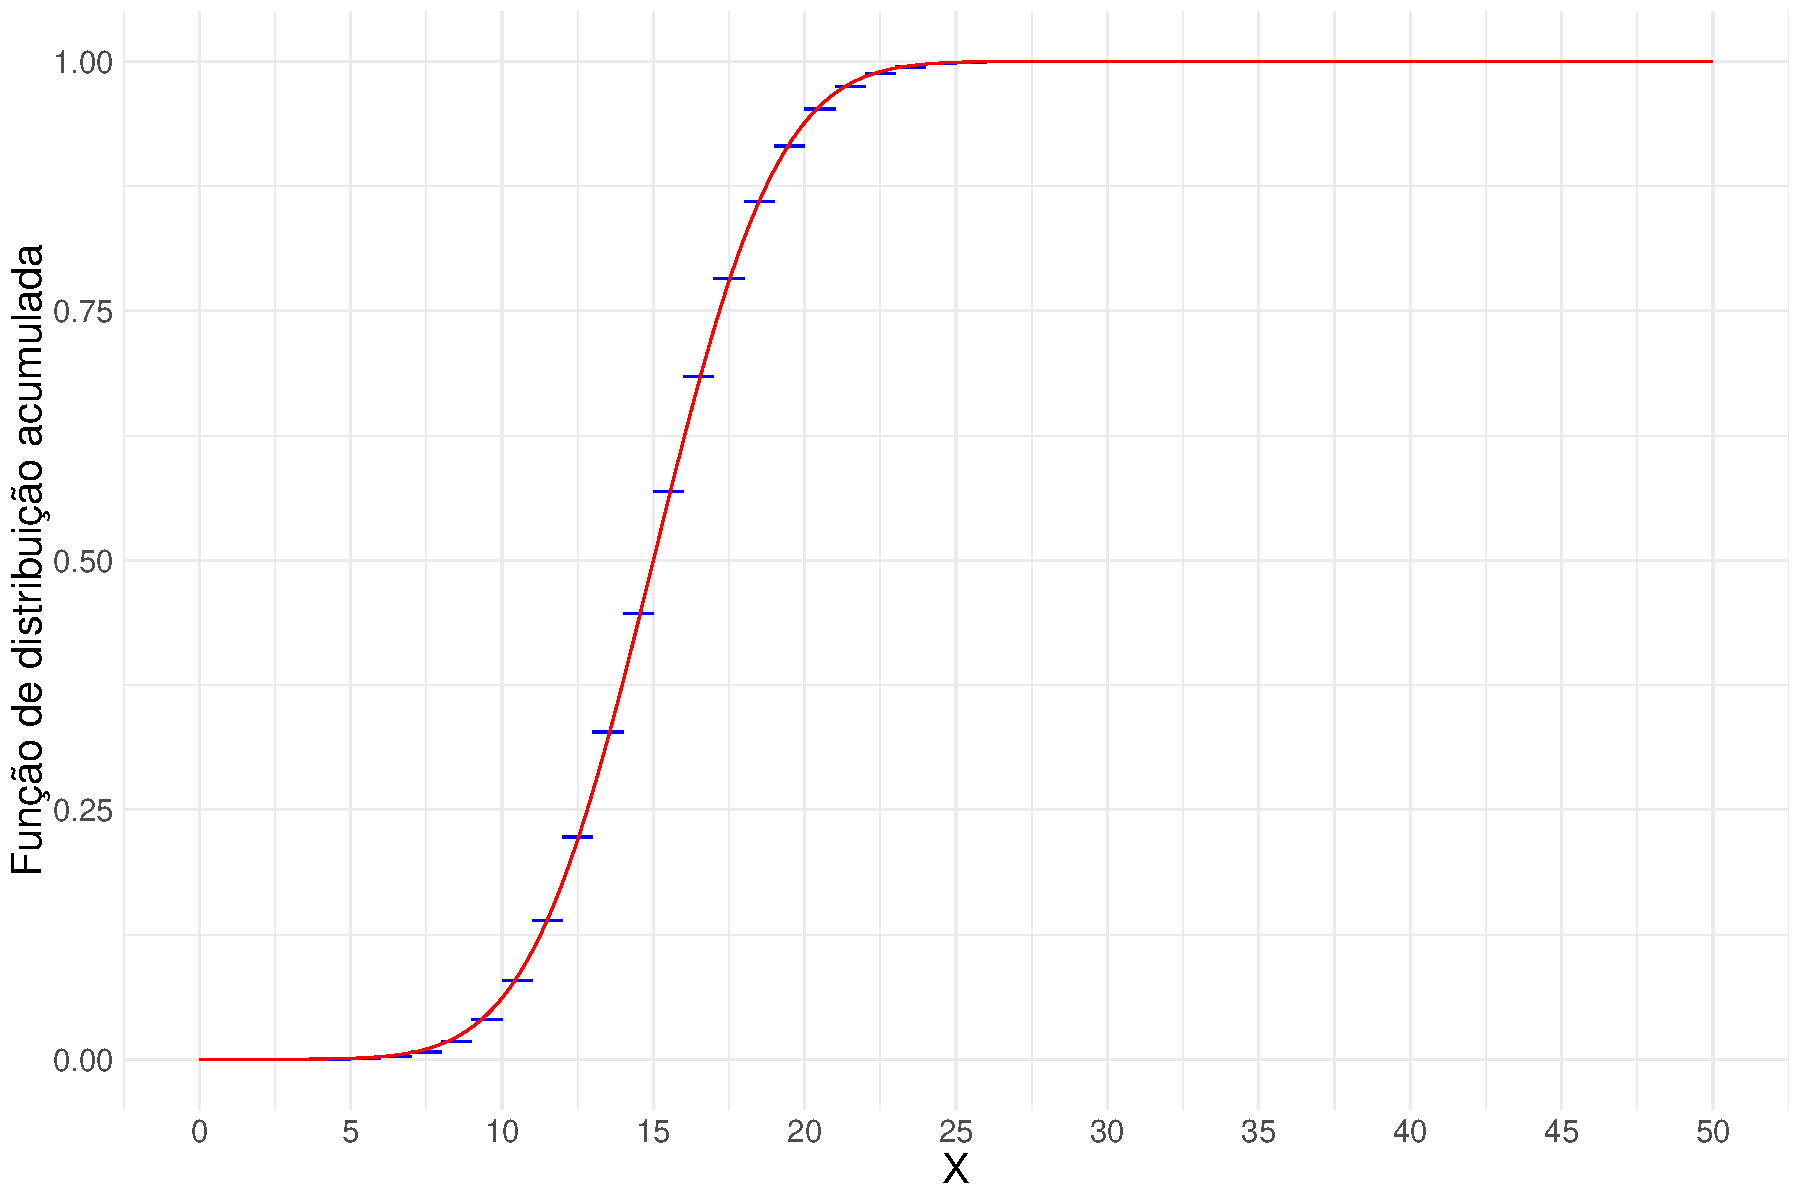
\includegraphics[width = 4.5cm]{figure/aproximacao.pdf}
 \end{figure}

\begin{block}{Correção da continuidade}
 {\scriptsize
  Consiste em alterar em $0,5$ unidade o valor que se deseja aproximar a função de distribuição acumulada. Mais especificamente, para $X \sim b(n; p)$
  \begin{align*}
   F(x) = P(X \leq x) \approx P( Y \leq x + 0,5) \qquad \mbox{ e } \qquad
   f(x) = P(X = x) \approx P(x - 0,5 \leq Y \leq x +0,5)
  \end{align*}

 }
\end{block}

\end{frame}

\begin{frame} {Exemplo}
 Estudo do Sindicato dos Bancários indica que cerca de 30\% dos funcionários do banco têm problemas de estresse, provenientes das condições de trabalho. Numa amostra de 200 bancários, qual seria a probabilidade de pelo menos 50 com essa doença?
 \vfill
 
 \textbf{Solução:}
 
 Note que $X \sim b(200; 0.3)$ com $\espe[X] = 200\cdot 0.3 = 60$ e $\vari(X) = 200\cdot 0.3 \cdot 0.7 = 42$, então
 \begin{align*}
  P(X \geq 50) &= 1 - P(X < 50) \\
  &= 1 - P(X \leq 49)\\
  &\approx 1 - P(Y \leq 49,5)\\
  &= 1 - \Phi\left( \dfrac{49,5 - 60}{\sqrt{42}} \right)\\
  &= 1 - \Phi(-1,62)\\
  &= 0,9474
 \end{align*}

 Observe que $P(X \geq 50) = 1 - P(X \leq 49) = 0,9494$.
\end{frame}



\section{Distribuição amostral}

\begin{frame}{Distribuição amostral: motivação}

{\scriptsize
Imagine que um professor tem uma turma com 30 alunos. As notas finais destes 30 alunos estão na Tabela~\ref{tab:dist_amostral}. Este professor está com tempo limitado e decidiu analisar o desempenho de 5 alunos ao final do curso. Existem $142.506$ maneiras de selecionar esses cinco alunos. Na Tabela~\ref{tab:amostras}, mostramos dez amostras diferentes com cinco alunos. Note que cada amostra tem uma média diferente. \textcolor{blue}{A ideia é que a média é uma variável (valor diferente em cada amostra) que denotamos por $\bar{X}$}.


\begin{table}[ht]
	\centering
	\begin{tabular}{cccccccccc}
		\toprule[0.05cm]
		7,29 & 7,19 & 7,15 & 5,54 & 5,93 & 5,53 & 6,44 & 6,27 & 8,16 & 5,72 \\ 
		4,84 & 4,63 & 6,11 & 7,10 & 3,37 & 7,36 & 6,70 & 5,70 & 6,31 & 7,64 \\ 
		5,89 & 8,82 & 7,77 & 7,93 & 5,24 & 6,08 & 5,77 & 6,57 & 6,00 & 6,14 \\ 
		\bottomrule[0.05cm]
	\end{tabular}
	\caption{Turma com 30 alunos.} 
	\label{tab:dist_amostral}
\end{table}



\begin{table}[ht]
	\centering
	\begin{tabular}{l|ccccc|c}
		\toprule[0.05cm]
		Amostras & Aluno 1 & Aluno 2 & Aluno 3 & Aluno 4 & Aluno 5 & Média da amostra \\ 
		\midrule[0.05cm]
		Amostra 1 &7,19 & 8,82 & 5,54 & 6,70 & 6,11 & 6,87 \\ 
		Amostra 2 &7,36 & 4,84 & 6,31 & 6,27 & 7,29 & 6,41 \\ 
		Amostra 3 & 5,77 & 6,57 & 6,44 & 8,16 & 7,93 & 6,97 \\ 
		Amostra 4 & 6,44 & 7,29 & 5,77 & 3,37 & 6,11 & 5,80 \\ 
		Amostra 5 & 6,14 & 7,36 & 3,37 & 6,70 & 7,10 & 6,13 \\ 
		Amostra 6 & 8,82 & 6,31 & 7,36 & 5,77 & 5,72 & 6,80 \\ 
		Amostra 7 & 7,10 & 7,93 & 4,84 & 6,44 & 5,93 & 6,45 \\ 
		Amostra 8 & 7,10 & 5,72 & 7,36 & 5,77 & 4,84 & 6,16 \\ 
		Amostra 9 & 6,44 & 6,14 & 7,64 & 6,08 & 5,70 & 6,40 \\ 
		Amostra 10 & 6,00 & 7,77 & 5,53 & 5,24 & 7,15 & 6,34 \\ 
		\bottomrule[0.05cm]
	\end{tabular}
	\caption{Dez amostras com cinco alunos com a média.} 
	\label{tab:amostras}
\end{table}
}
\end{frame}

\begin{frame}{Distribuição amostral de médias de notas.}

\begin{figure}
	\centering
	\subcaptionbox{$n=5$\label{fig:cont5}}{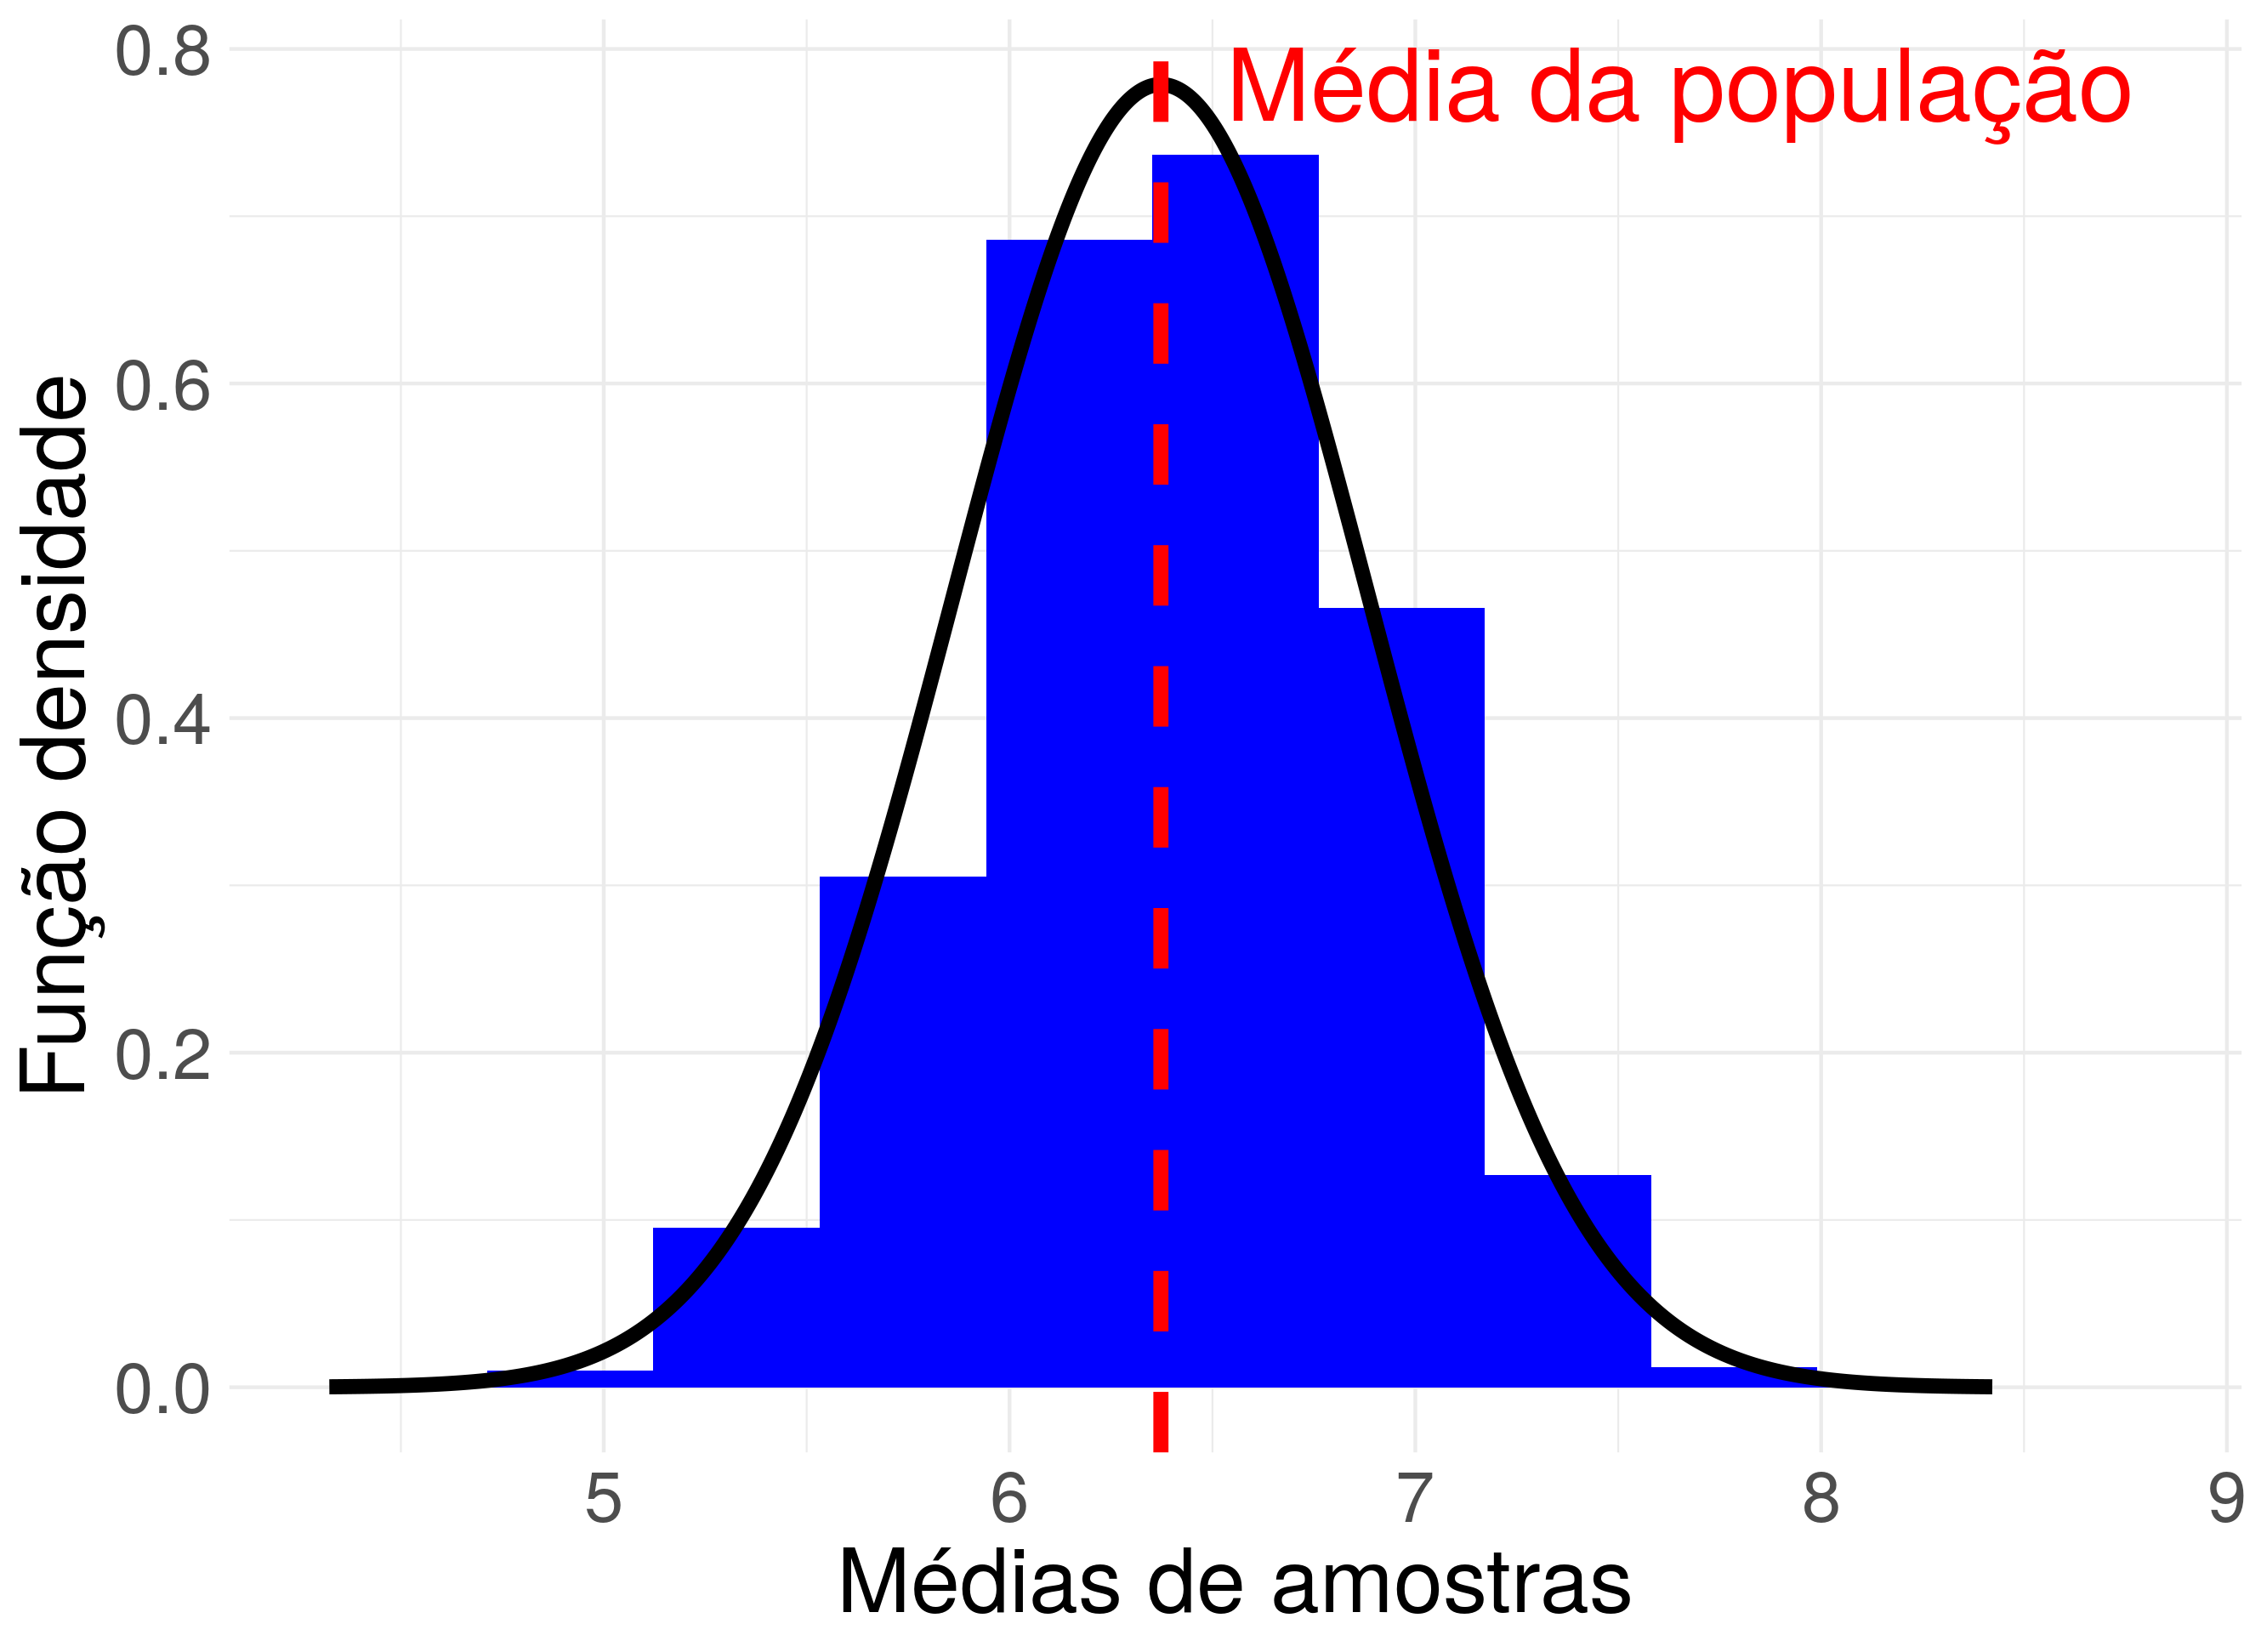
\includegraphics[width=0.3\linewidth]{figure/amostras_notas_5.png}} \hspace{2.5cm}
	\subcaptionbox{$n=25$\label{fig:cont25}}{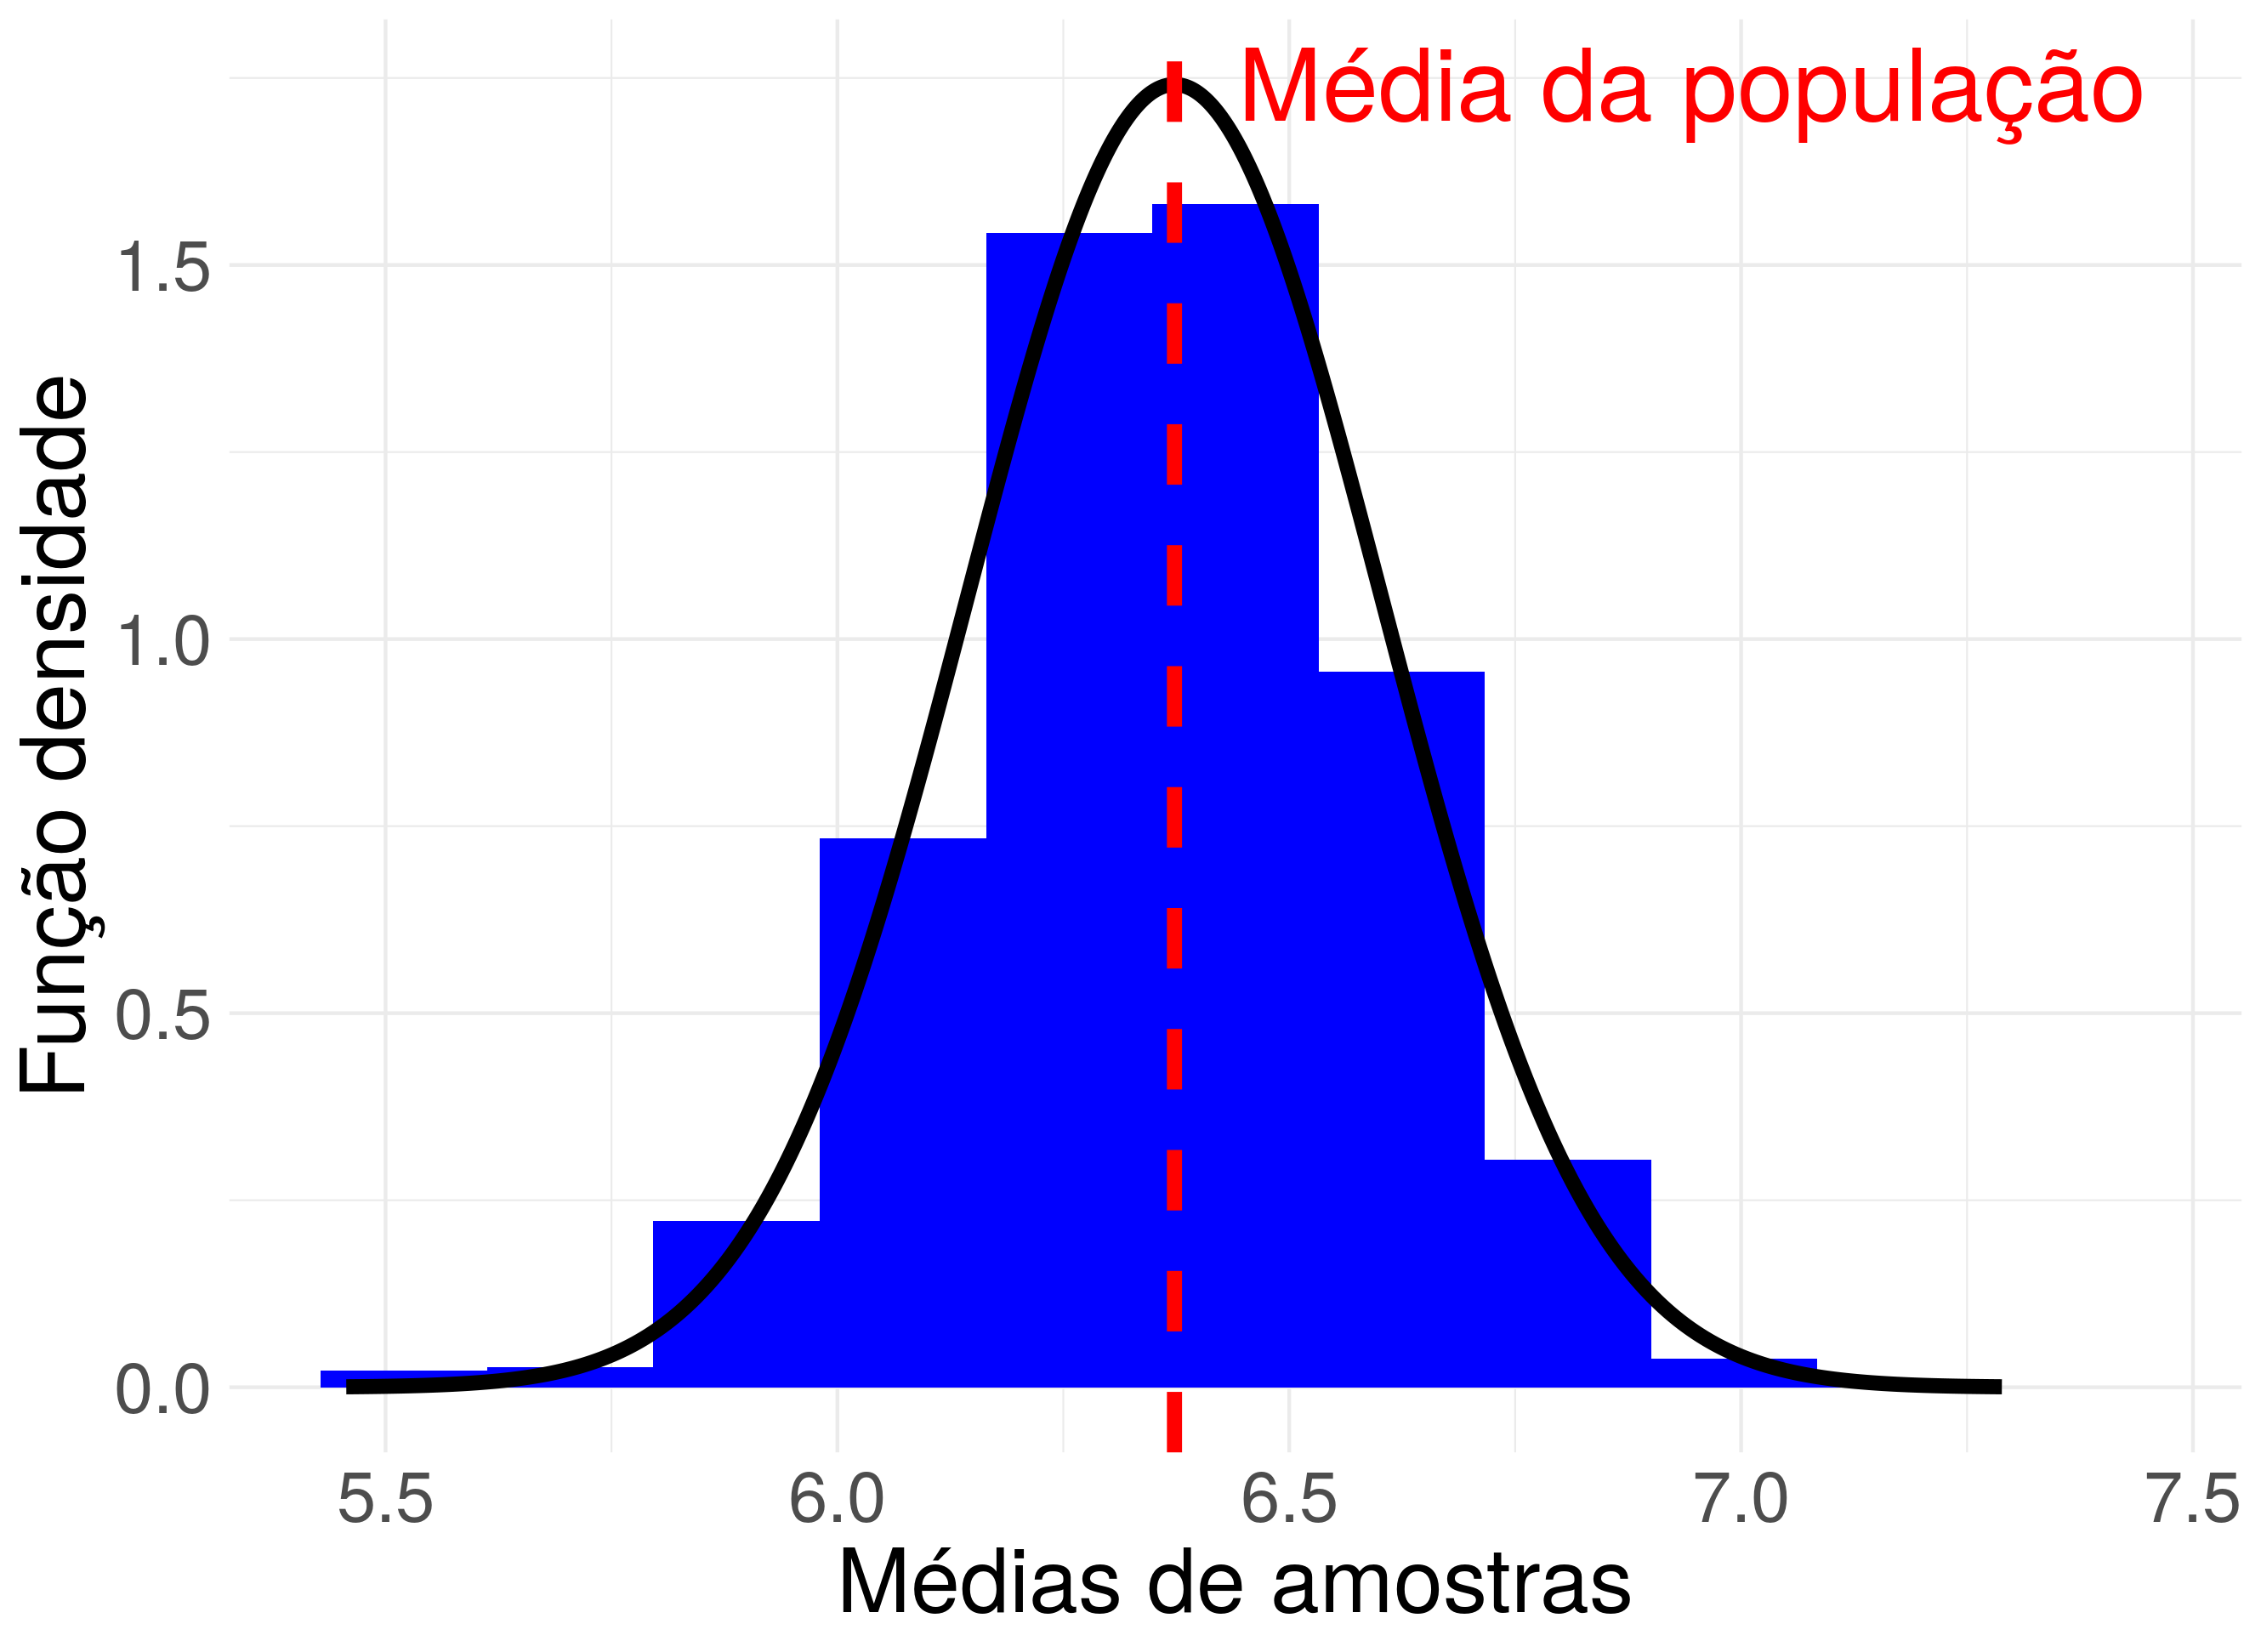
\includegraphics[width=.3\linewidth]{figure/amostras_notas_25.png}} \\
	\subcaptionbox{$n=50$\label{fig:cont50}}{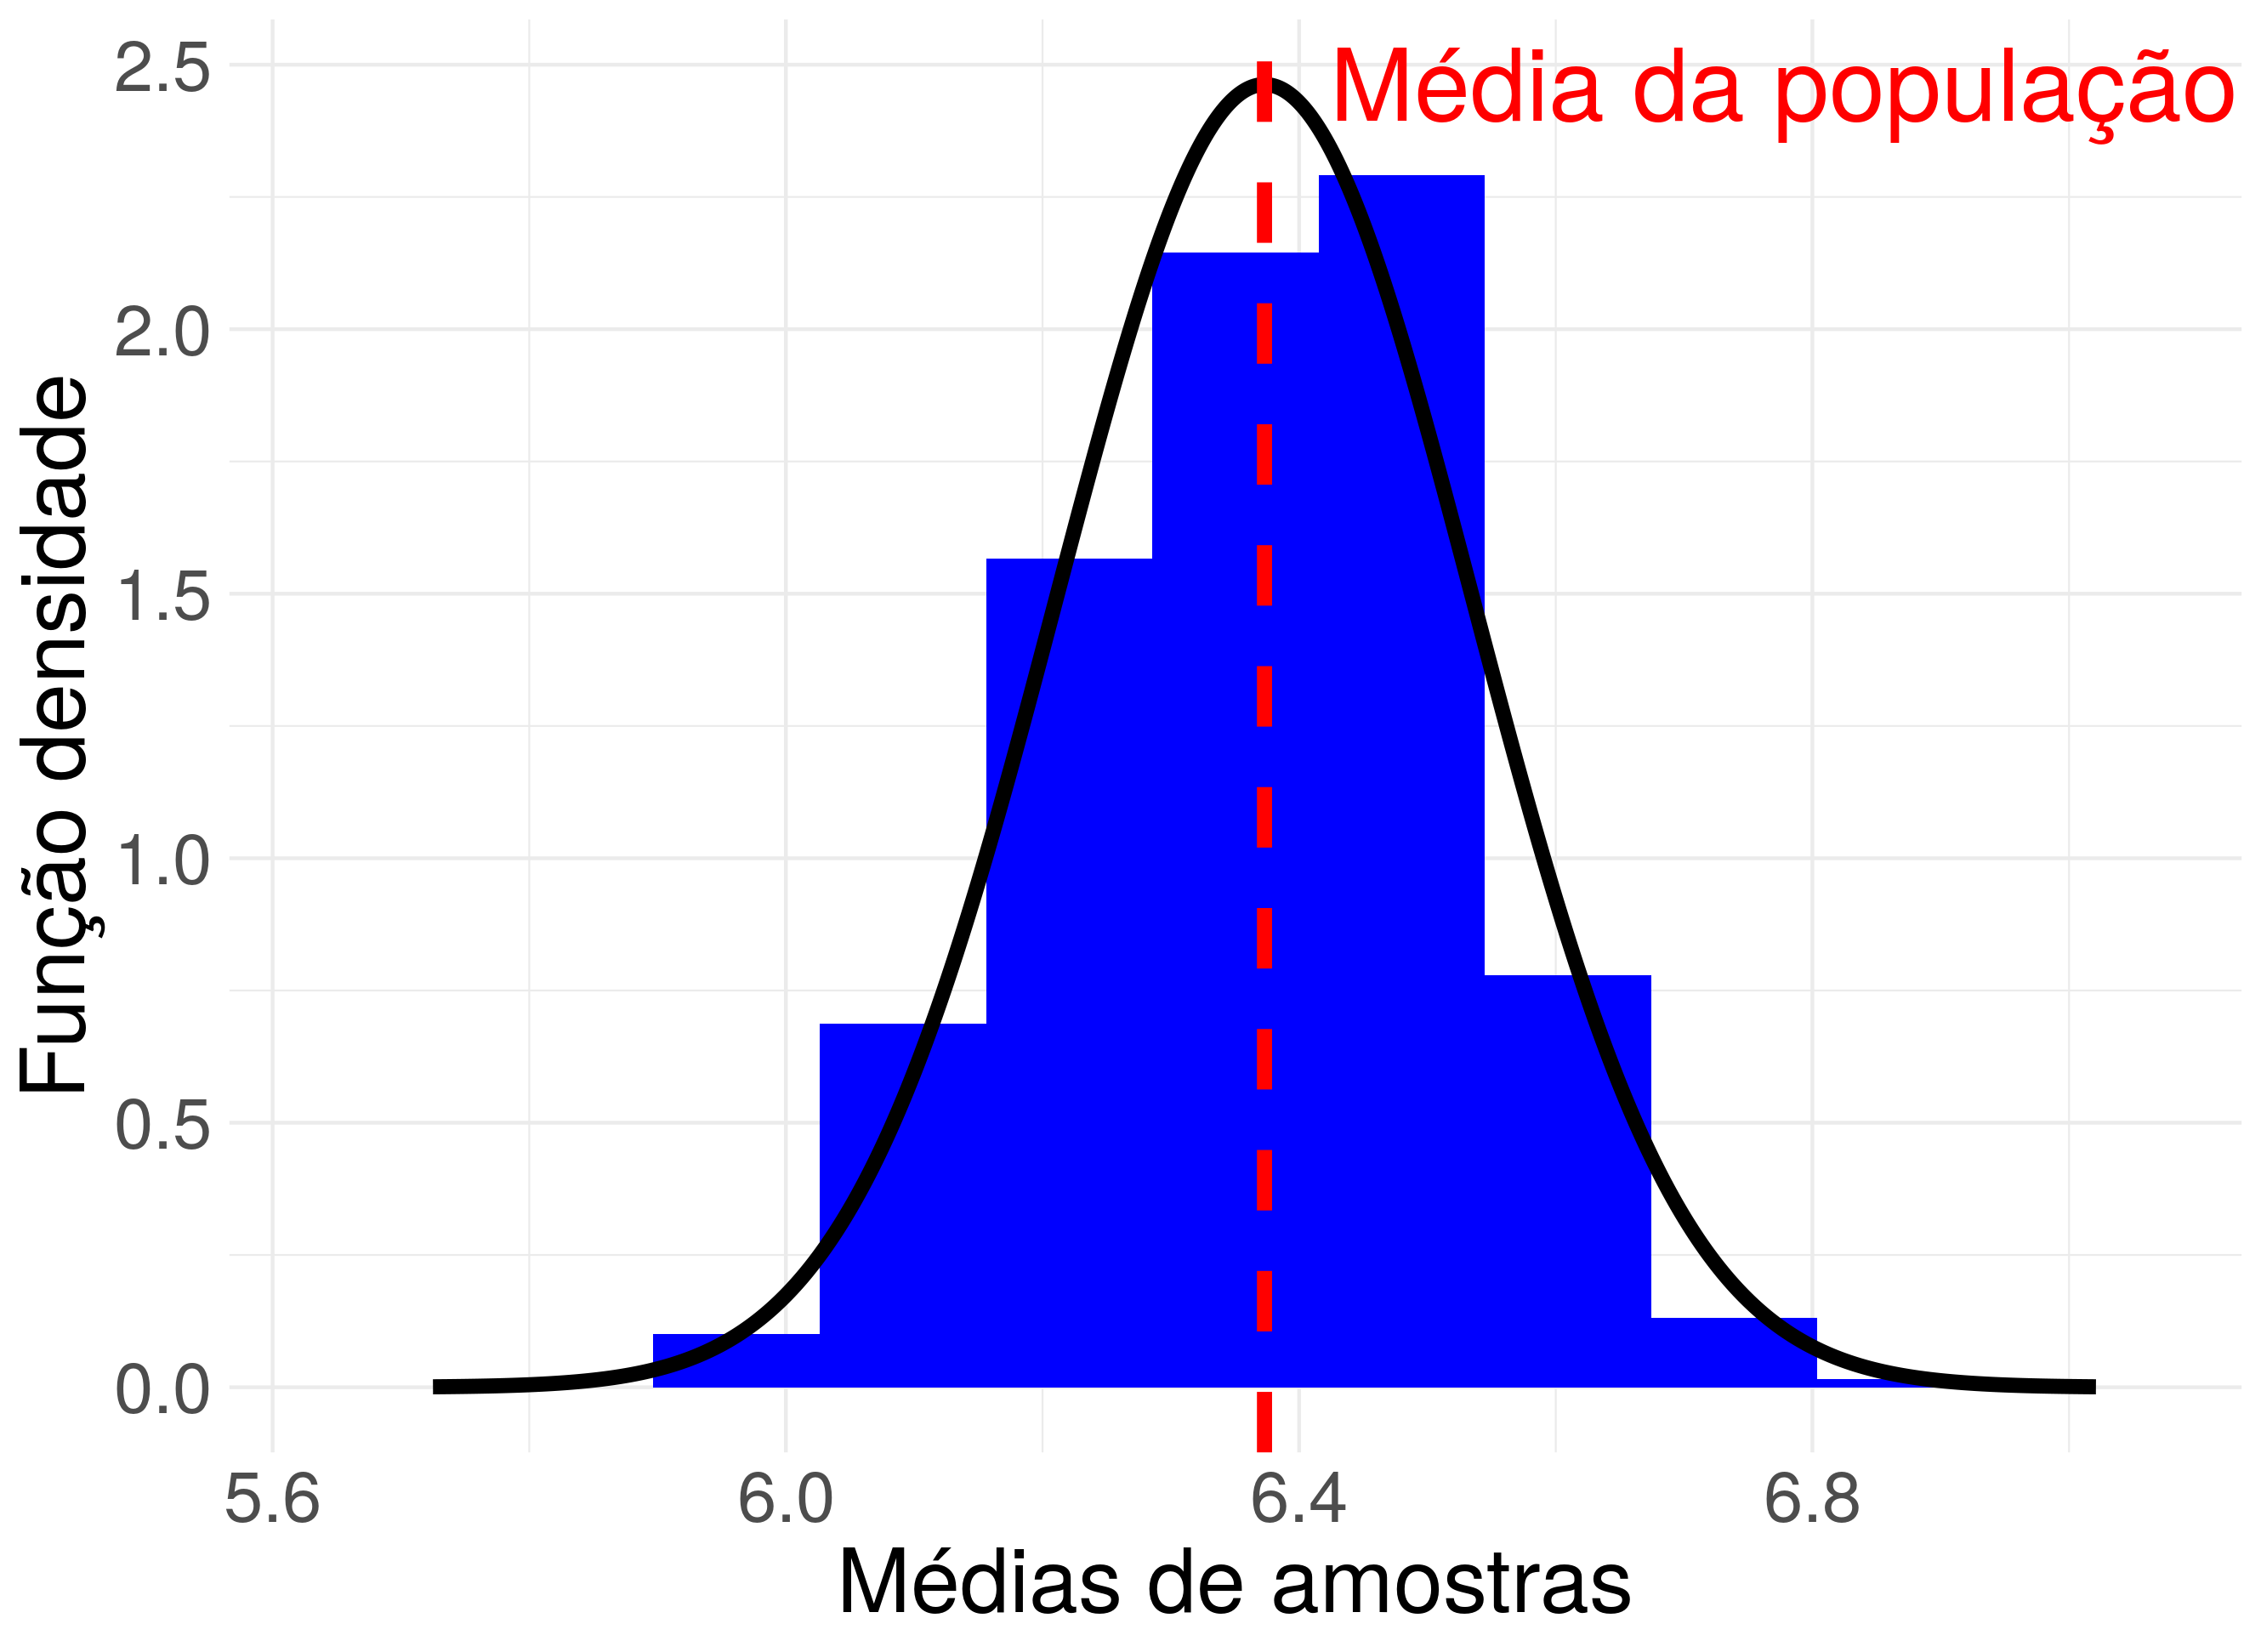
\includegraphics[width=0.3\linewidth]{figure/amostras_notas_50.png}} \hspace{2.5cm}
	\subcaptionbox{$n=75$\label{fig:cont75}}{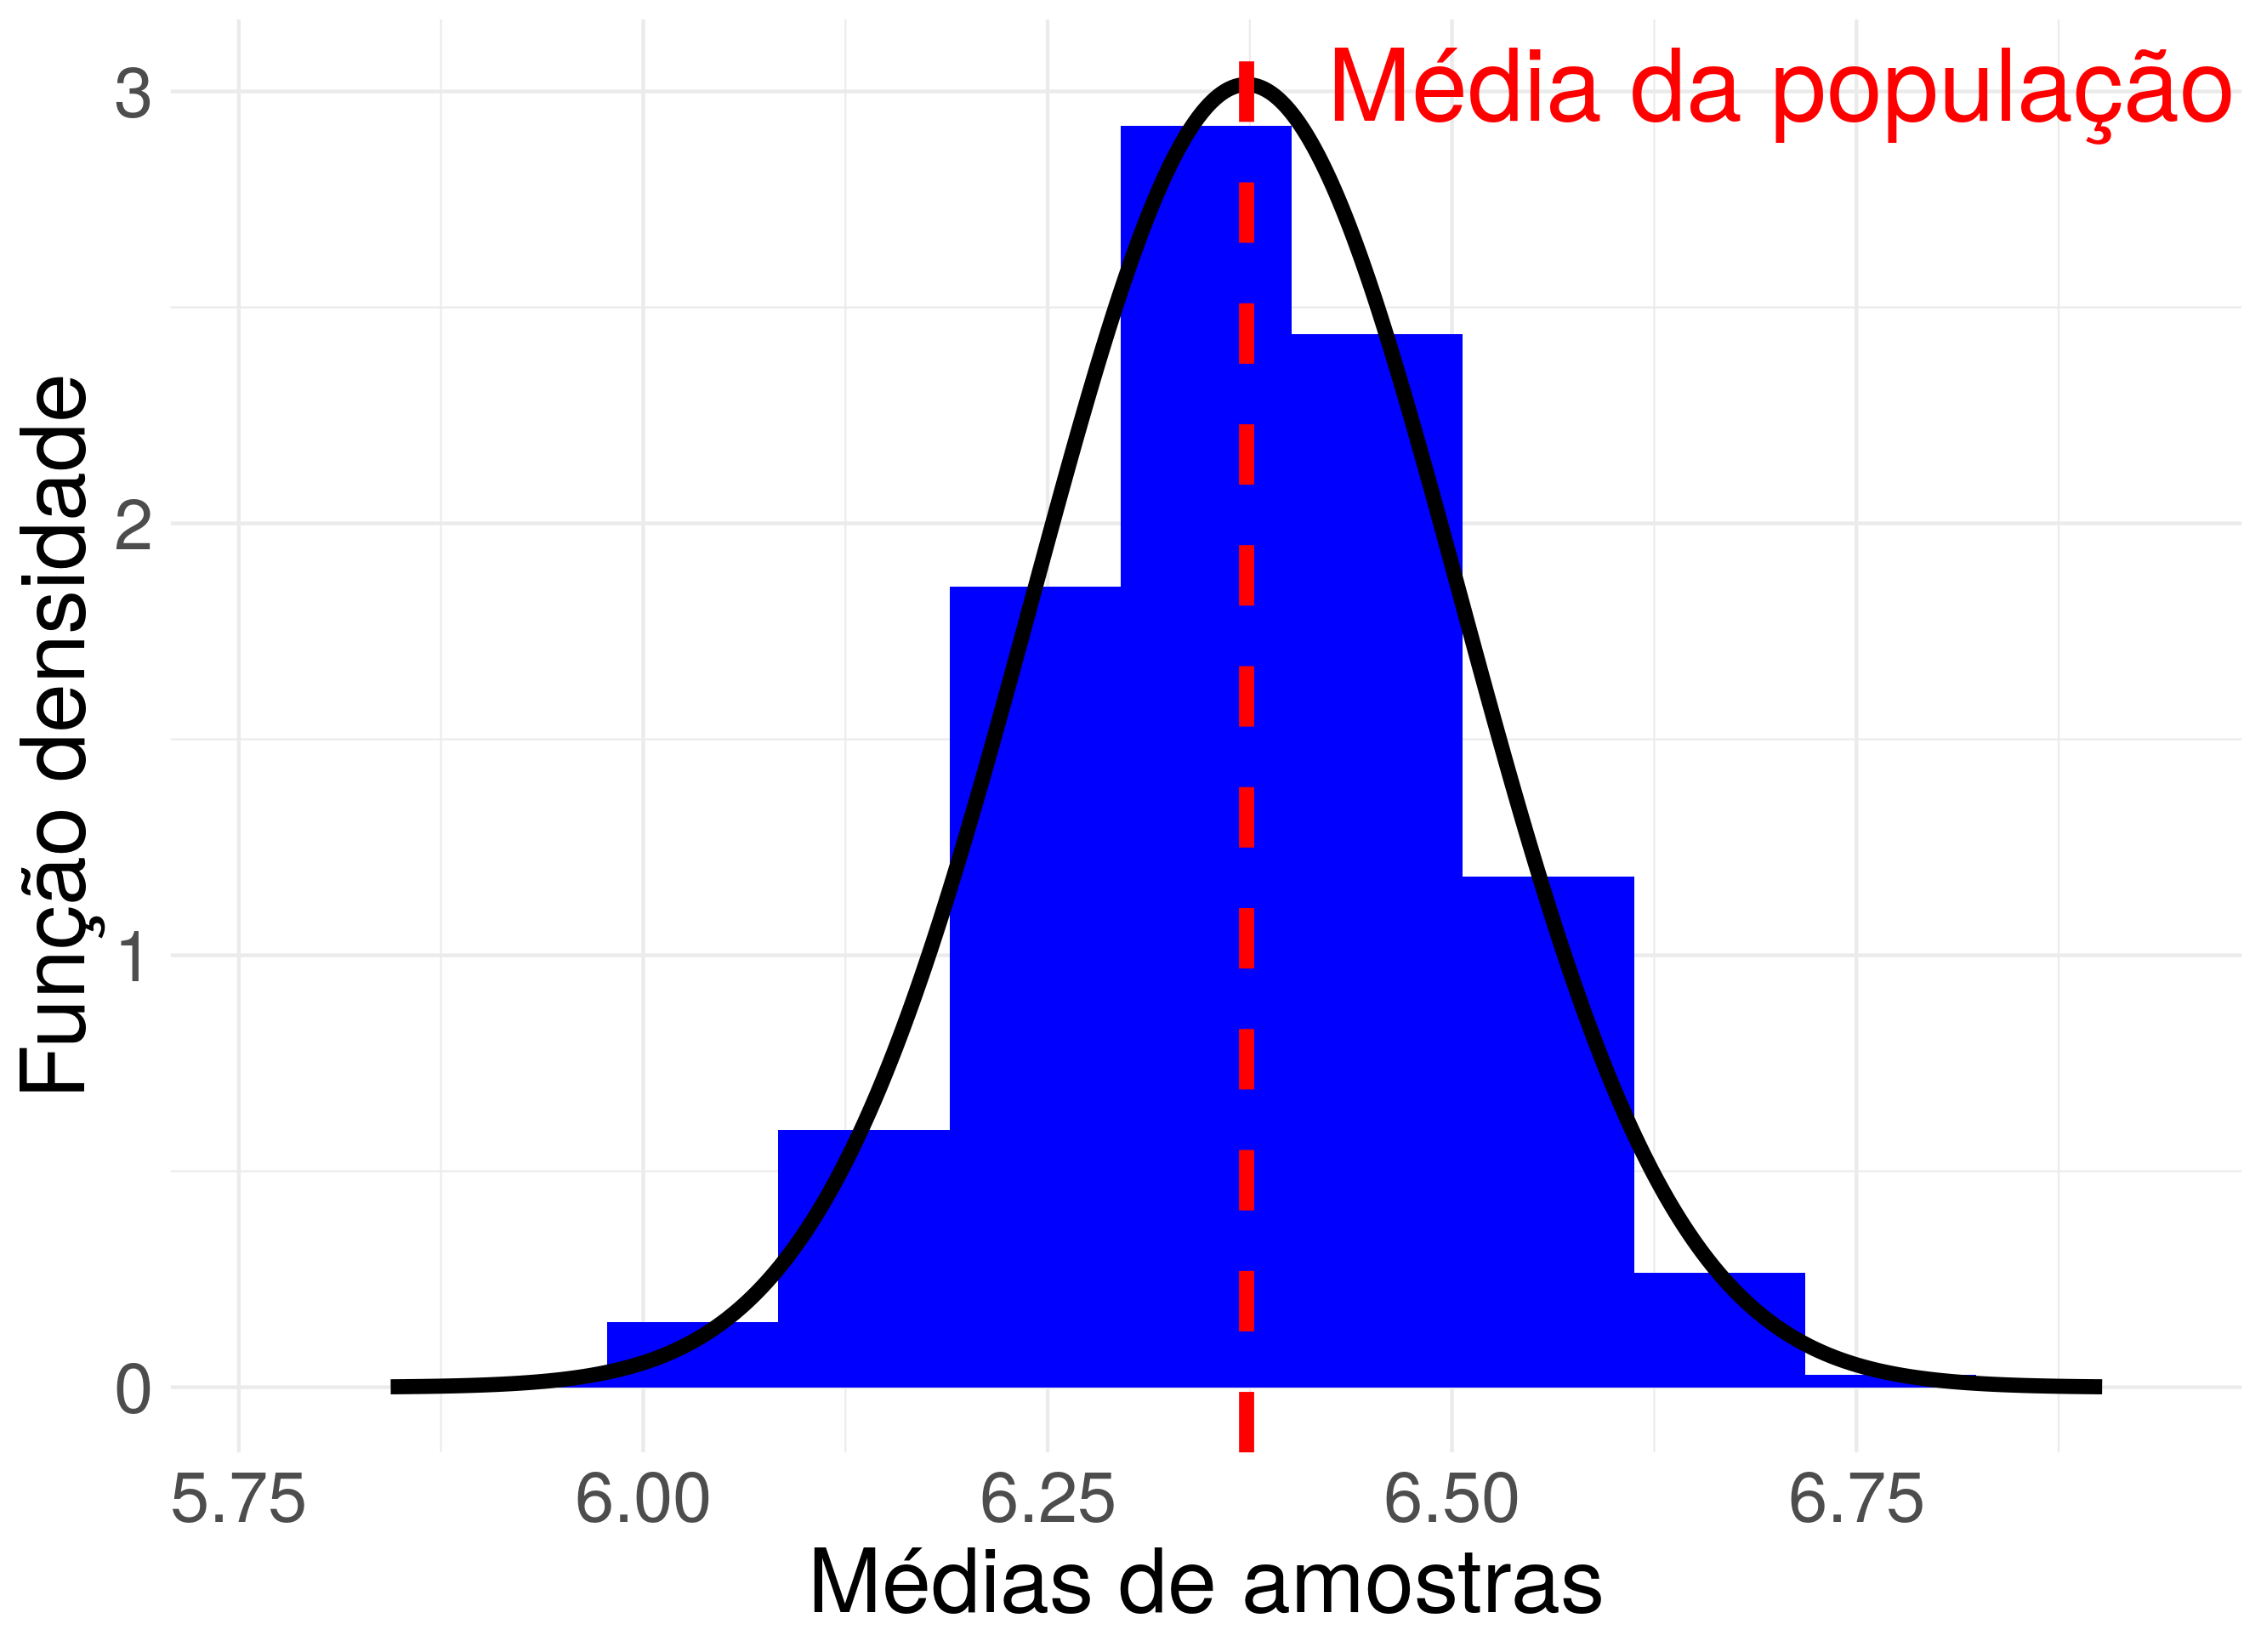
\includegraphics[width=.3\linewidth]{figure/amostras_notas_75.png}}
	\caption{Médias das amostras: demonstração do teorema central do limite.}
	\label{fig:medias_cont}
\end{figure}
	
\end{frame}



\begin{frame}{Distribuição amostral: motivação}

Considere a variável discreta $X$ com suporte e função de probabilidade dada pela Tabela~\ref{tab:var_X}. Na Tabela~\ref{tab:amostras_disc}, apresentamos dez amostras com cinco valores. Note que cada amostra tem uma média que não precisa ser um número inteiro. \textcolor{blue}{A ideia é que a média uma variável aleatória (valor diferente em cada amostra) que denotamos por $\bar{X}$.} 

\scriptsize

\begin{table}[htbp]
	\centering
	\caption{Variável discreta $X$ com suporte e função de probabilidade.}
	\label{tab:var_X}
	\begin{tabular}{l|cccccc}
		\toprule[0.05cm]
		$x$ & $0$ & $1$ & $2$ & $3$ & $4$ & $5$ \\ \midrule[0.05cm]
		$f(x)$ & $0,1$ & $0,4$ & $0,05$ & $0,05$ & $0,3$ & $0,1$ \\
		\bottomrule[0.05cm]
	\end{tabular}
\end{table}


	\begin{table}[ht]
		\centering
				\caption{Dez amostras de uma variável quantitativa.} 
		\label{tab:amostras_disc}
		\begin{tabular}{l|ccccc|c}
			\toprule[0.05cm]
		Amostras	& Valor 1 & Valor 2 & Valor 3 & Valor 4 & Valor 5 & Média \\ 
			\midrule[0.05cm]
			Amostra 1 & 4 & 1 & 1 & 4 & 1 & 2,20 \\ 
			Amostra 2 & 1 & 0 & 1 & 1 & 4 & 1,40 \\ 
			Amostra 3 & 4 & 4 & 5 & 3 & 4 & 4,00 \\ 
			Amostra 4 & 4 & 1 & 5 & 4 & 4 & 3,60 \\ 
			Amostra 5 & 4 & 5 & 1 & 4 & 1 & 3,00 \\ 
			Amostra 6 & 0 & 1 & 0 & 1 & 0 & 0,40 \\ 
			Amostra 7 & 5 & 4 & 4 & 4 & 1 & 3,60 \\ 
			Amostra 8 & 2 & 3 & 5 & 5 & 2 & 3,40 \\ 
			Amostra 9 & 4 & 4 & 3 & 4 & 1 & 3,20 \\ 
			Amostra 10 & 1 & 1 & 4 & 1 & 5 & 2,40 \\ 
			\bottomrule[0.05cm]
		\end{tabular}

	\end{table}

\normalsize
\end{frame}

\begin{frame}{Distribuição amostral de médias da variável discreta $X$.}

\begin{figure}
	\centering
	\subcaptionbox{$n=5$\label{fig:disc5}}{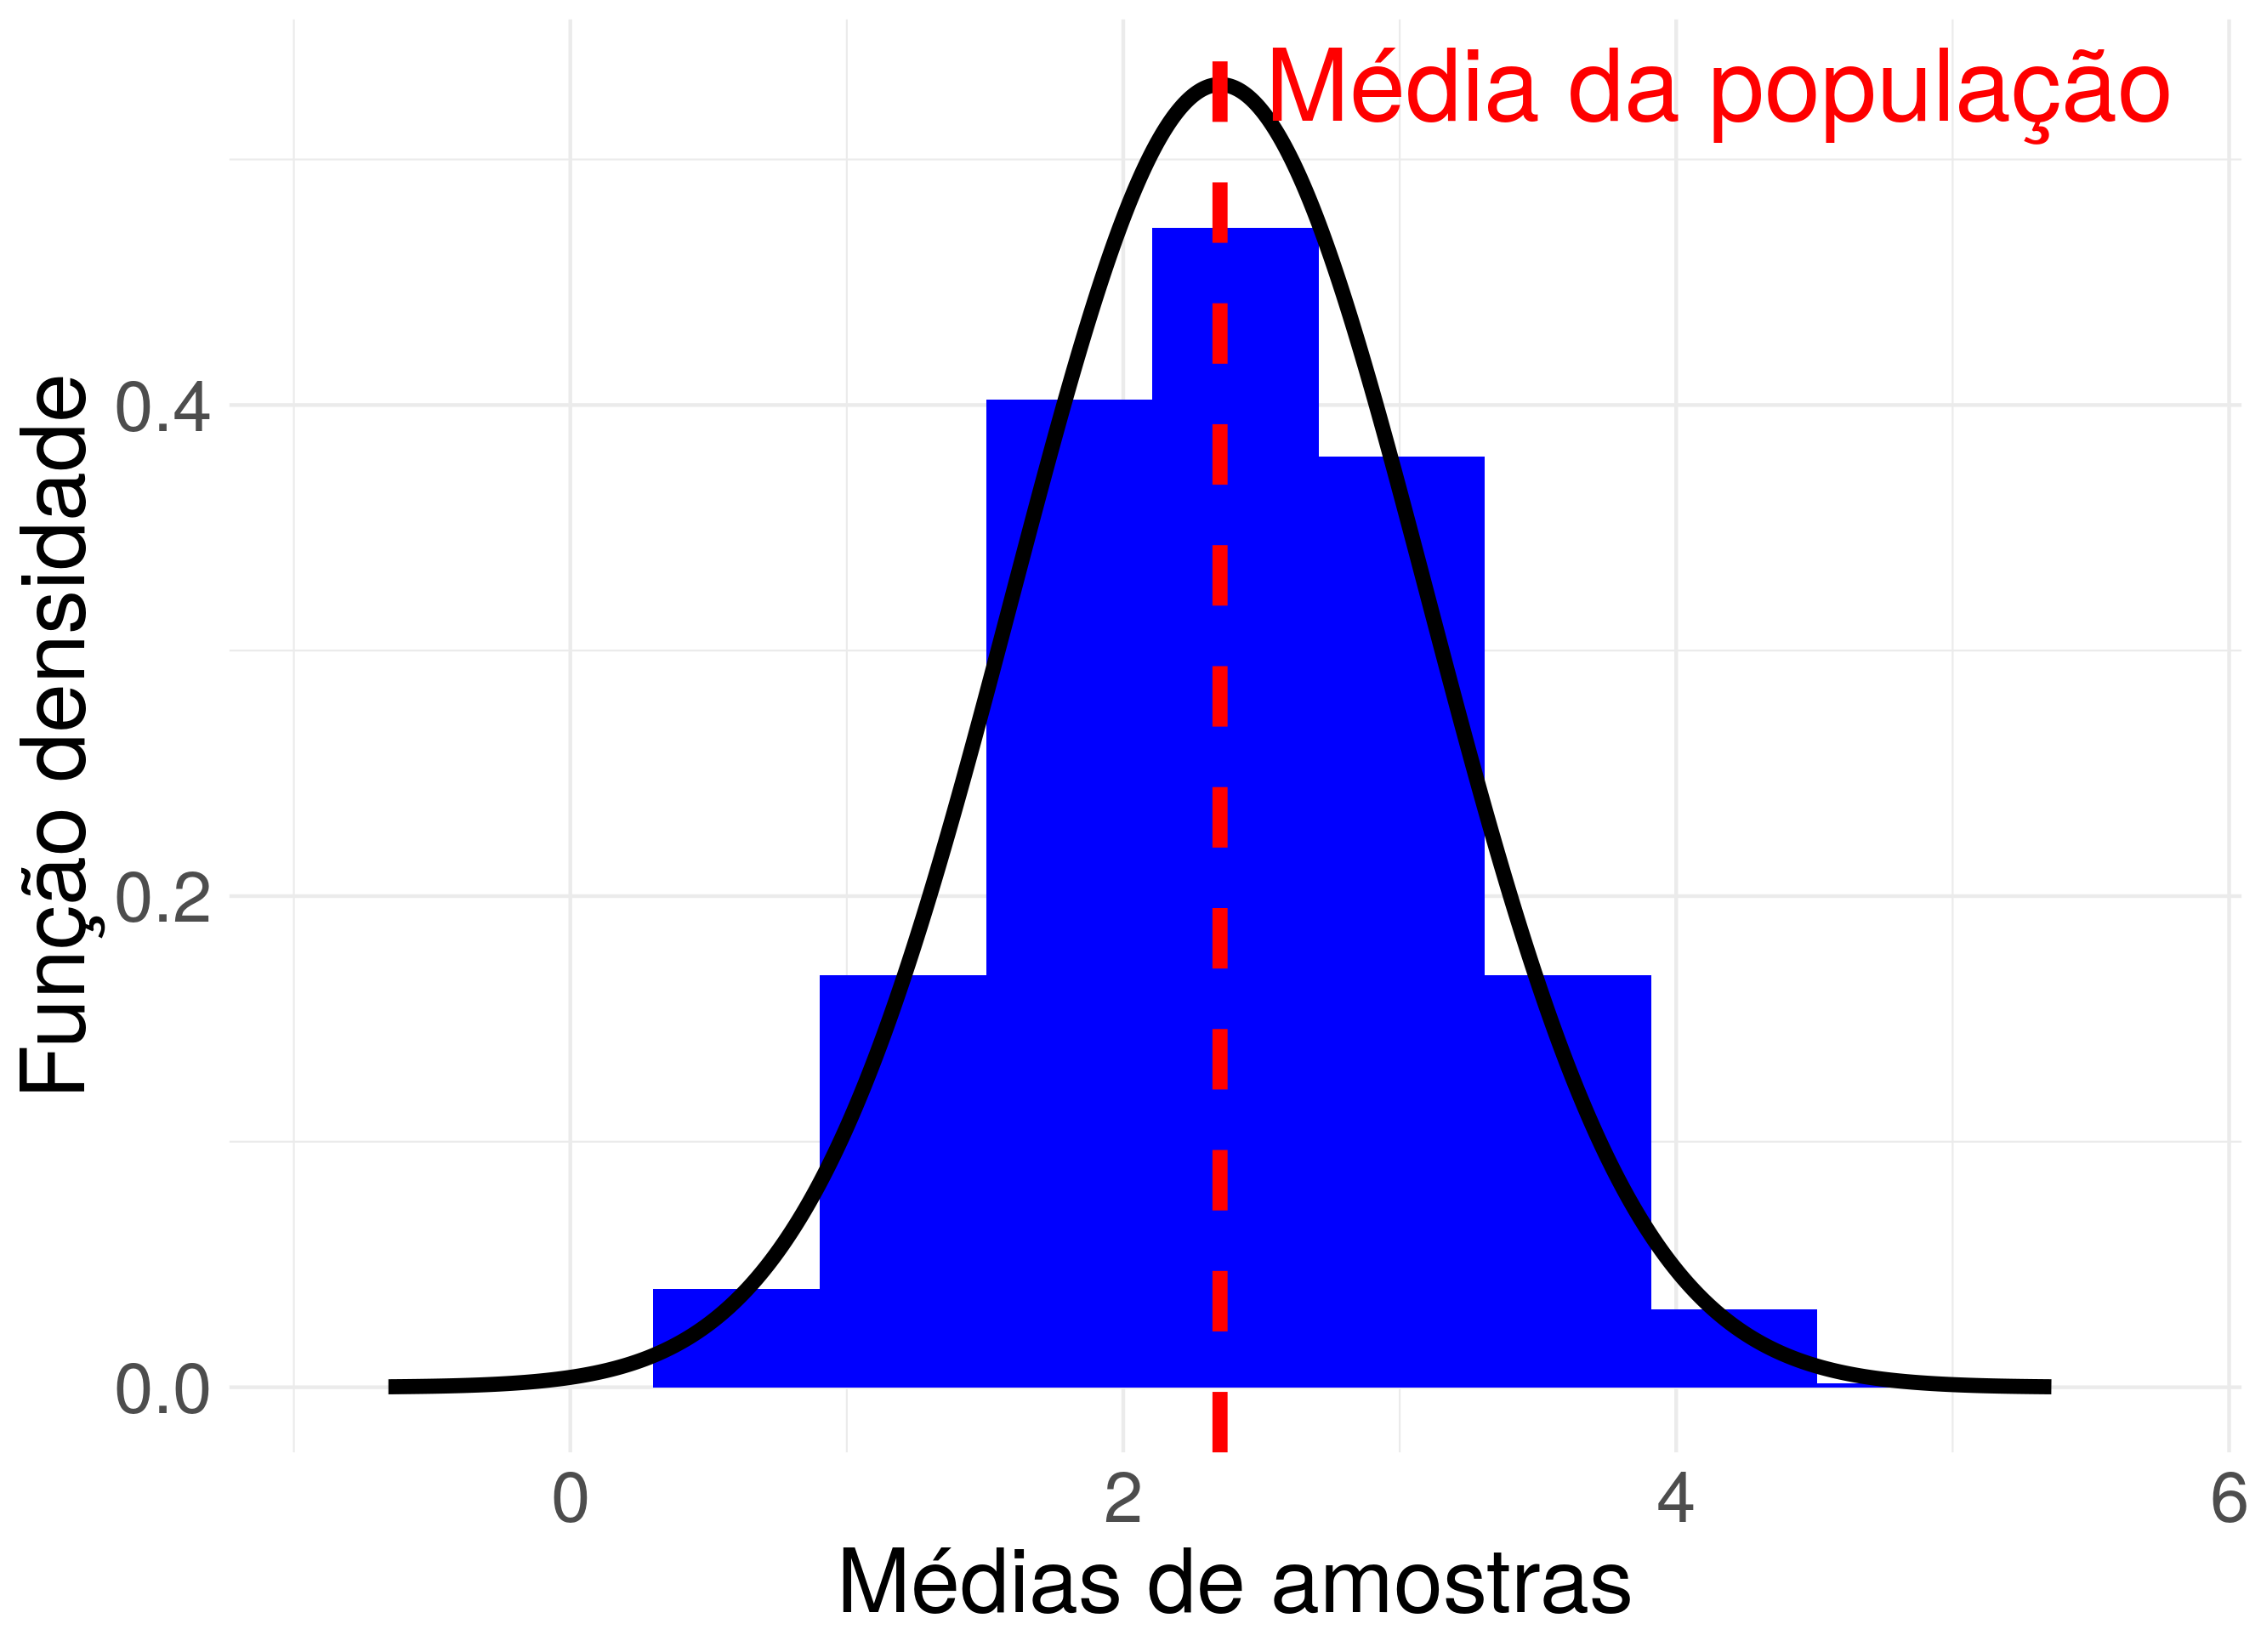
\includegraphics[width=0.3\linewidth]{figure/amostras_discreta_5.png}} \hspace{2.5cm}
	\subcaptionbox{$n=25$\label{fig:disc25}}{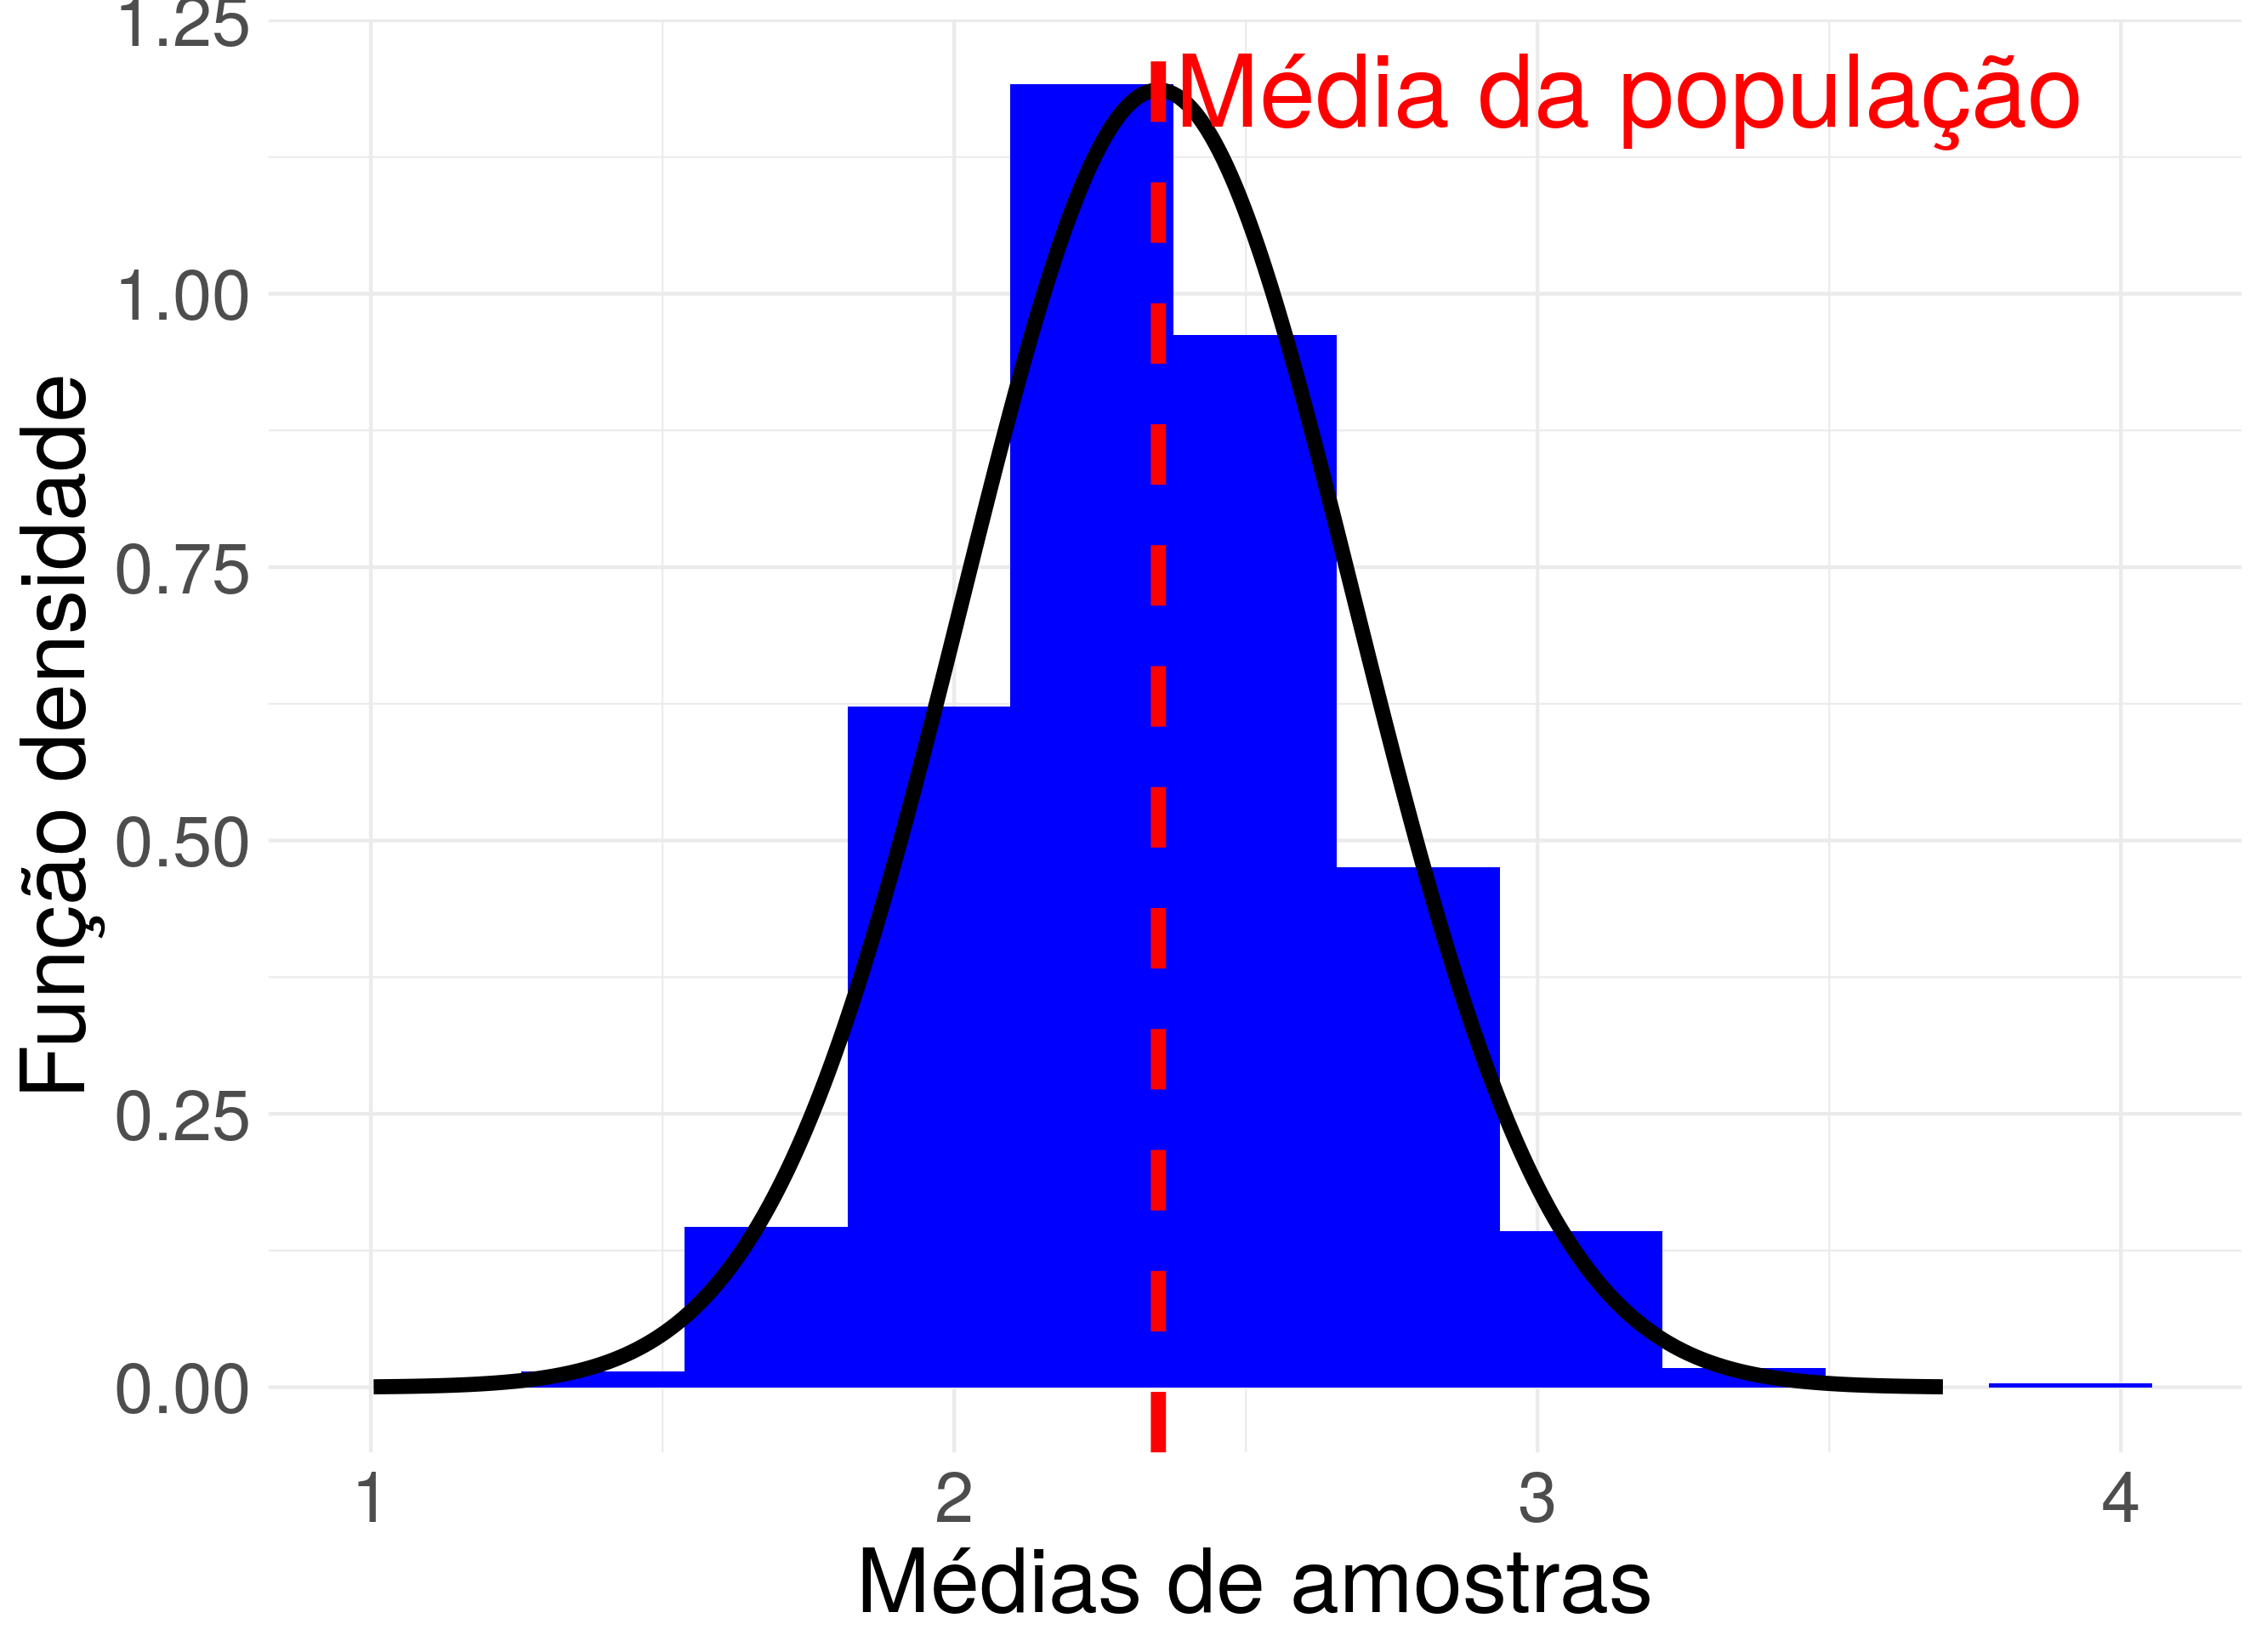
\includegraphics[width=.3\linewidth]{figure/amostras_discreta_25.png}} \\
	\subcaptionbox{$n=50$\label{fig:disc50}}{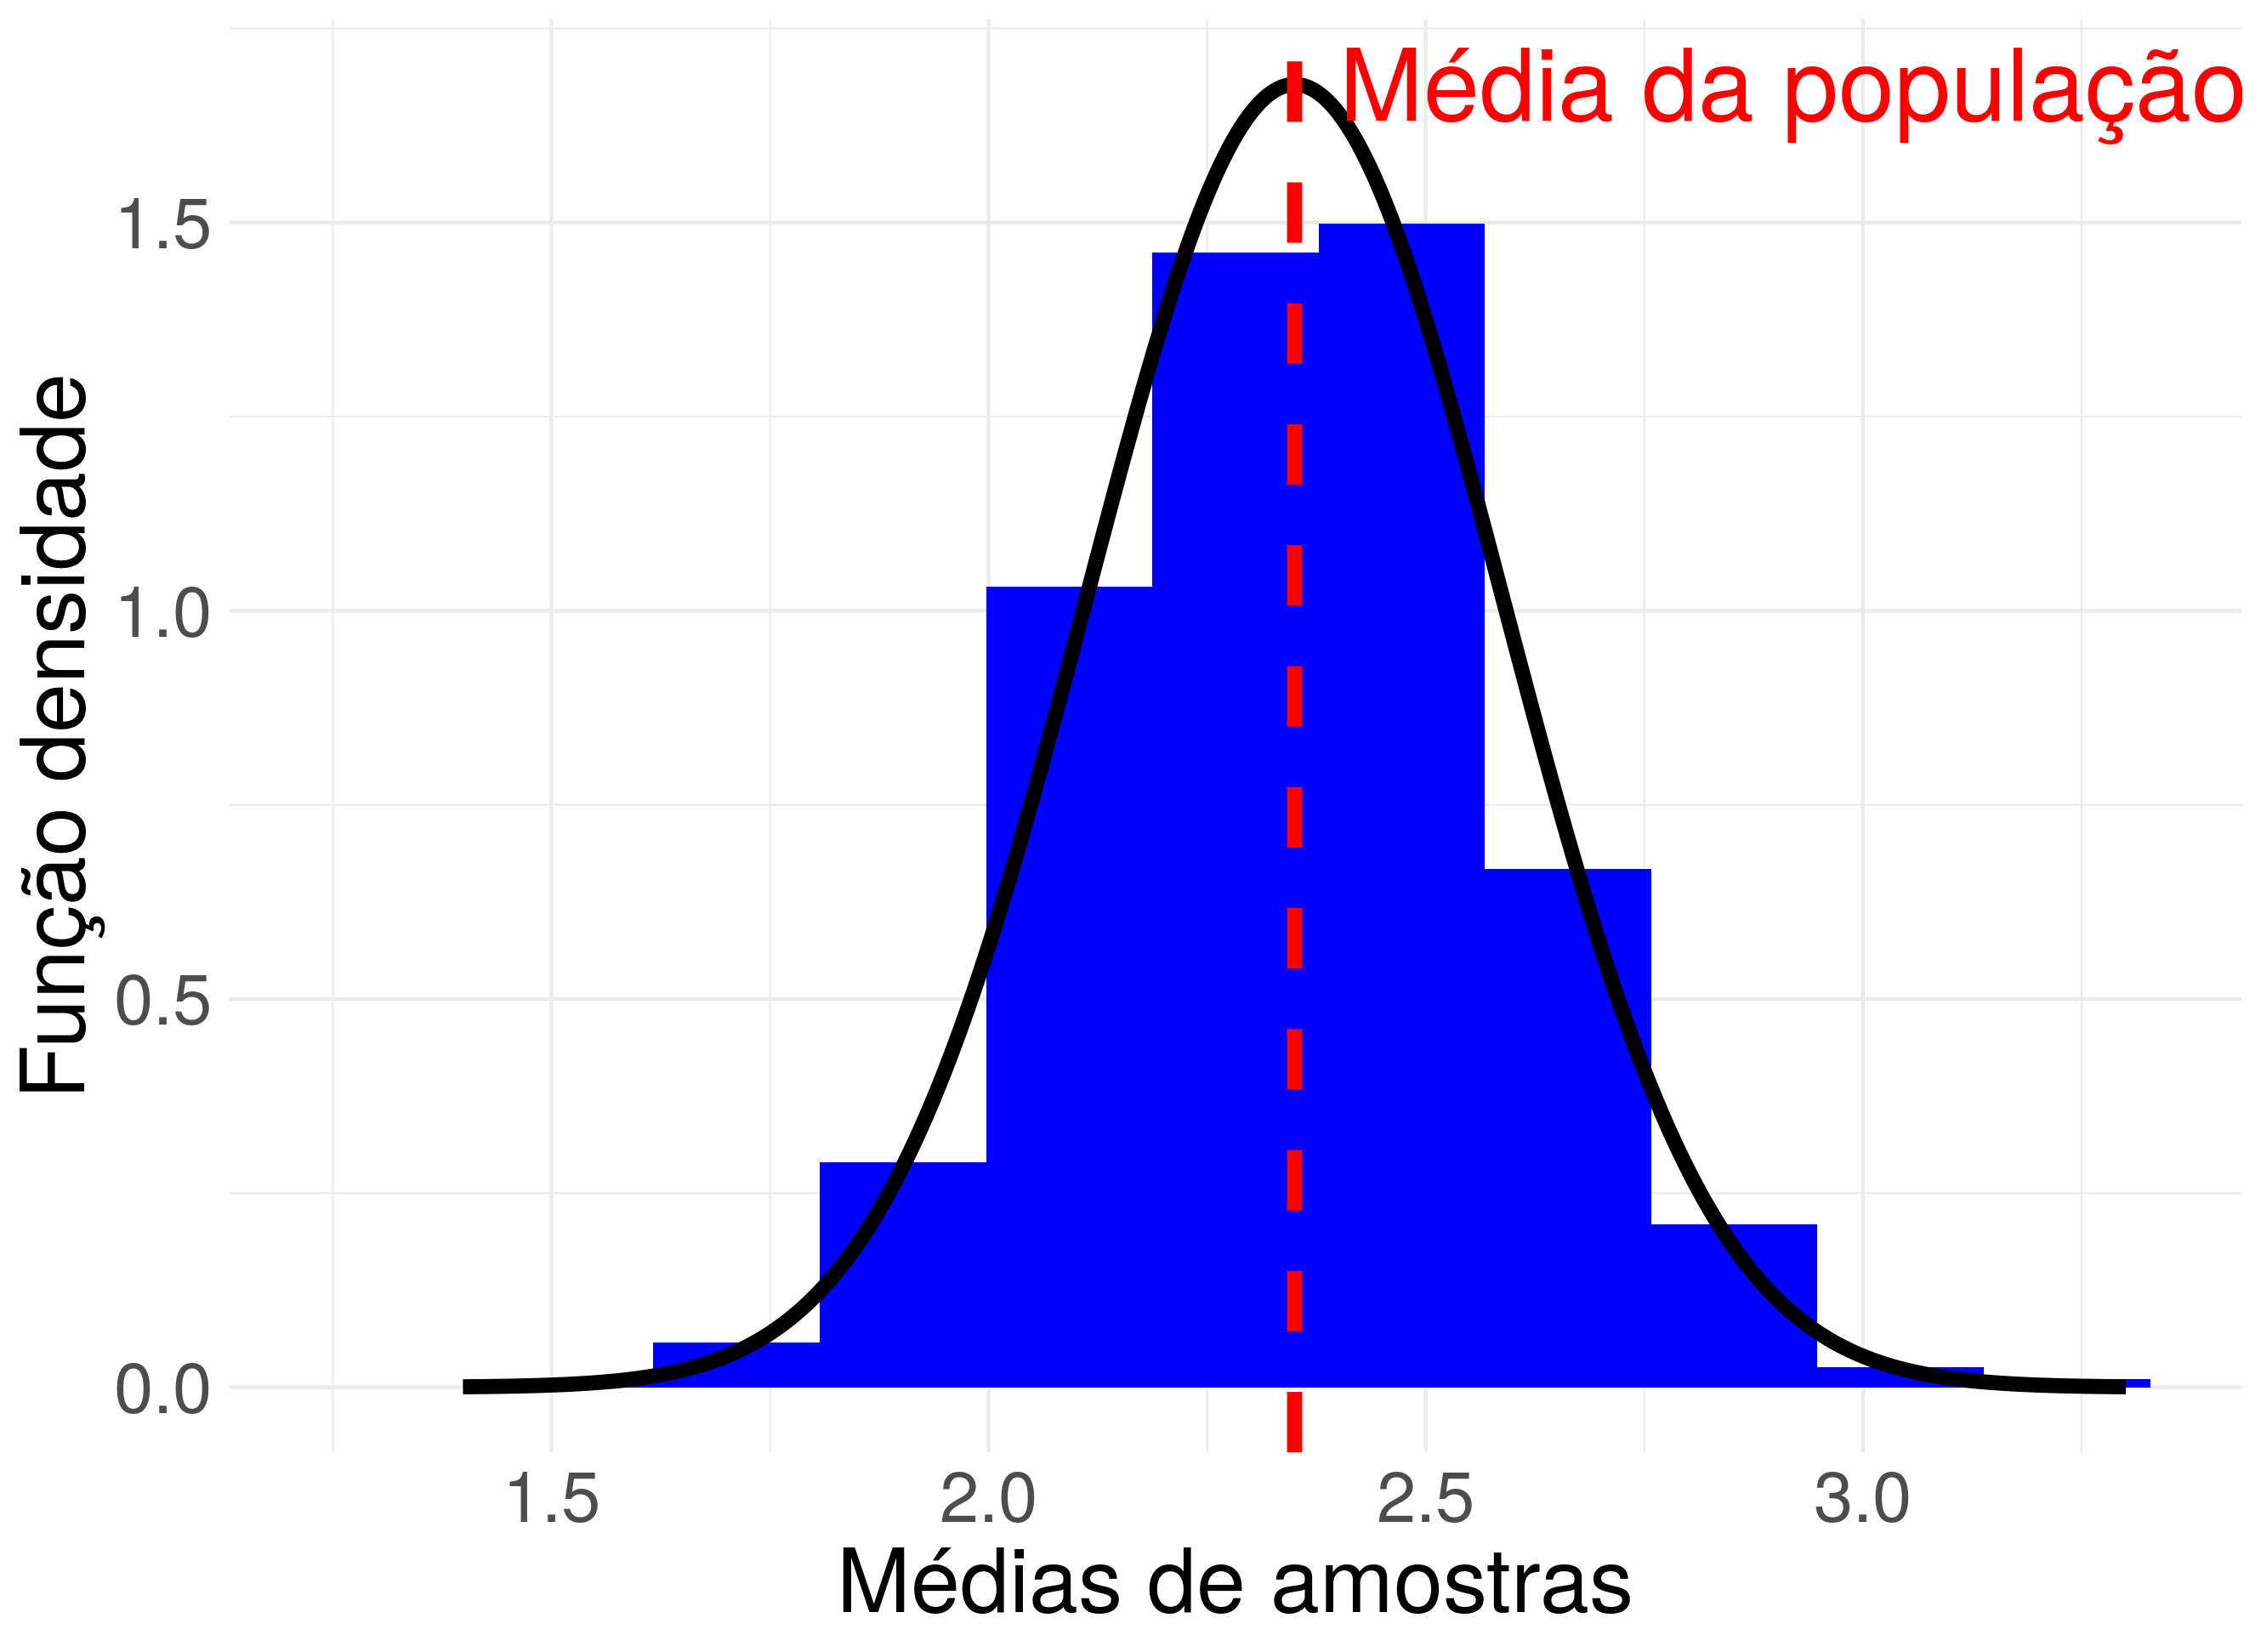
\includegraphics[width=0.3\linewidth]{figure/amostras_discreta_50.png}} \hspace{2.5cm}
	\subcaptionbox{$n=75$\label{fig:disc75}}{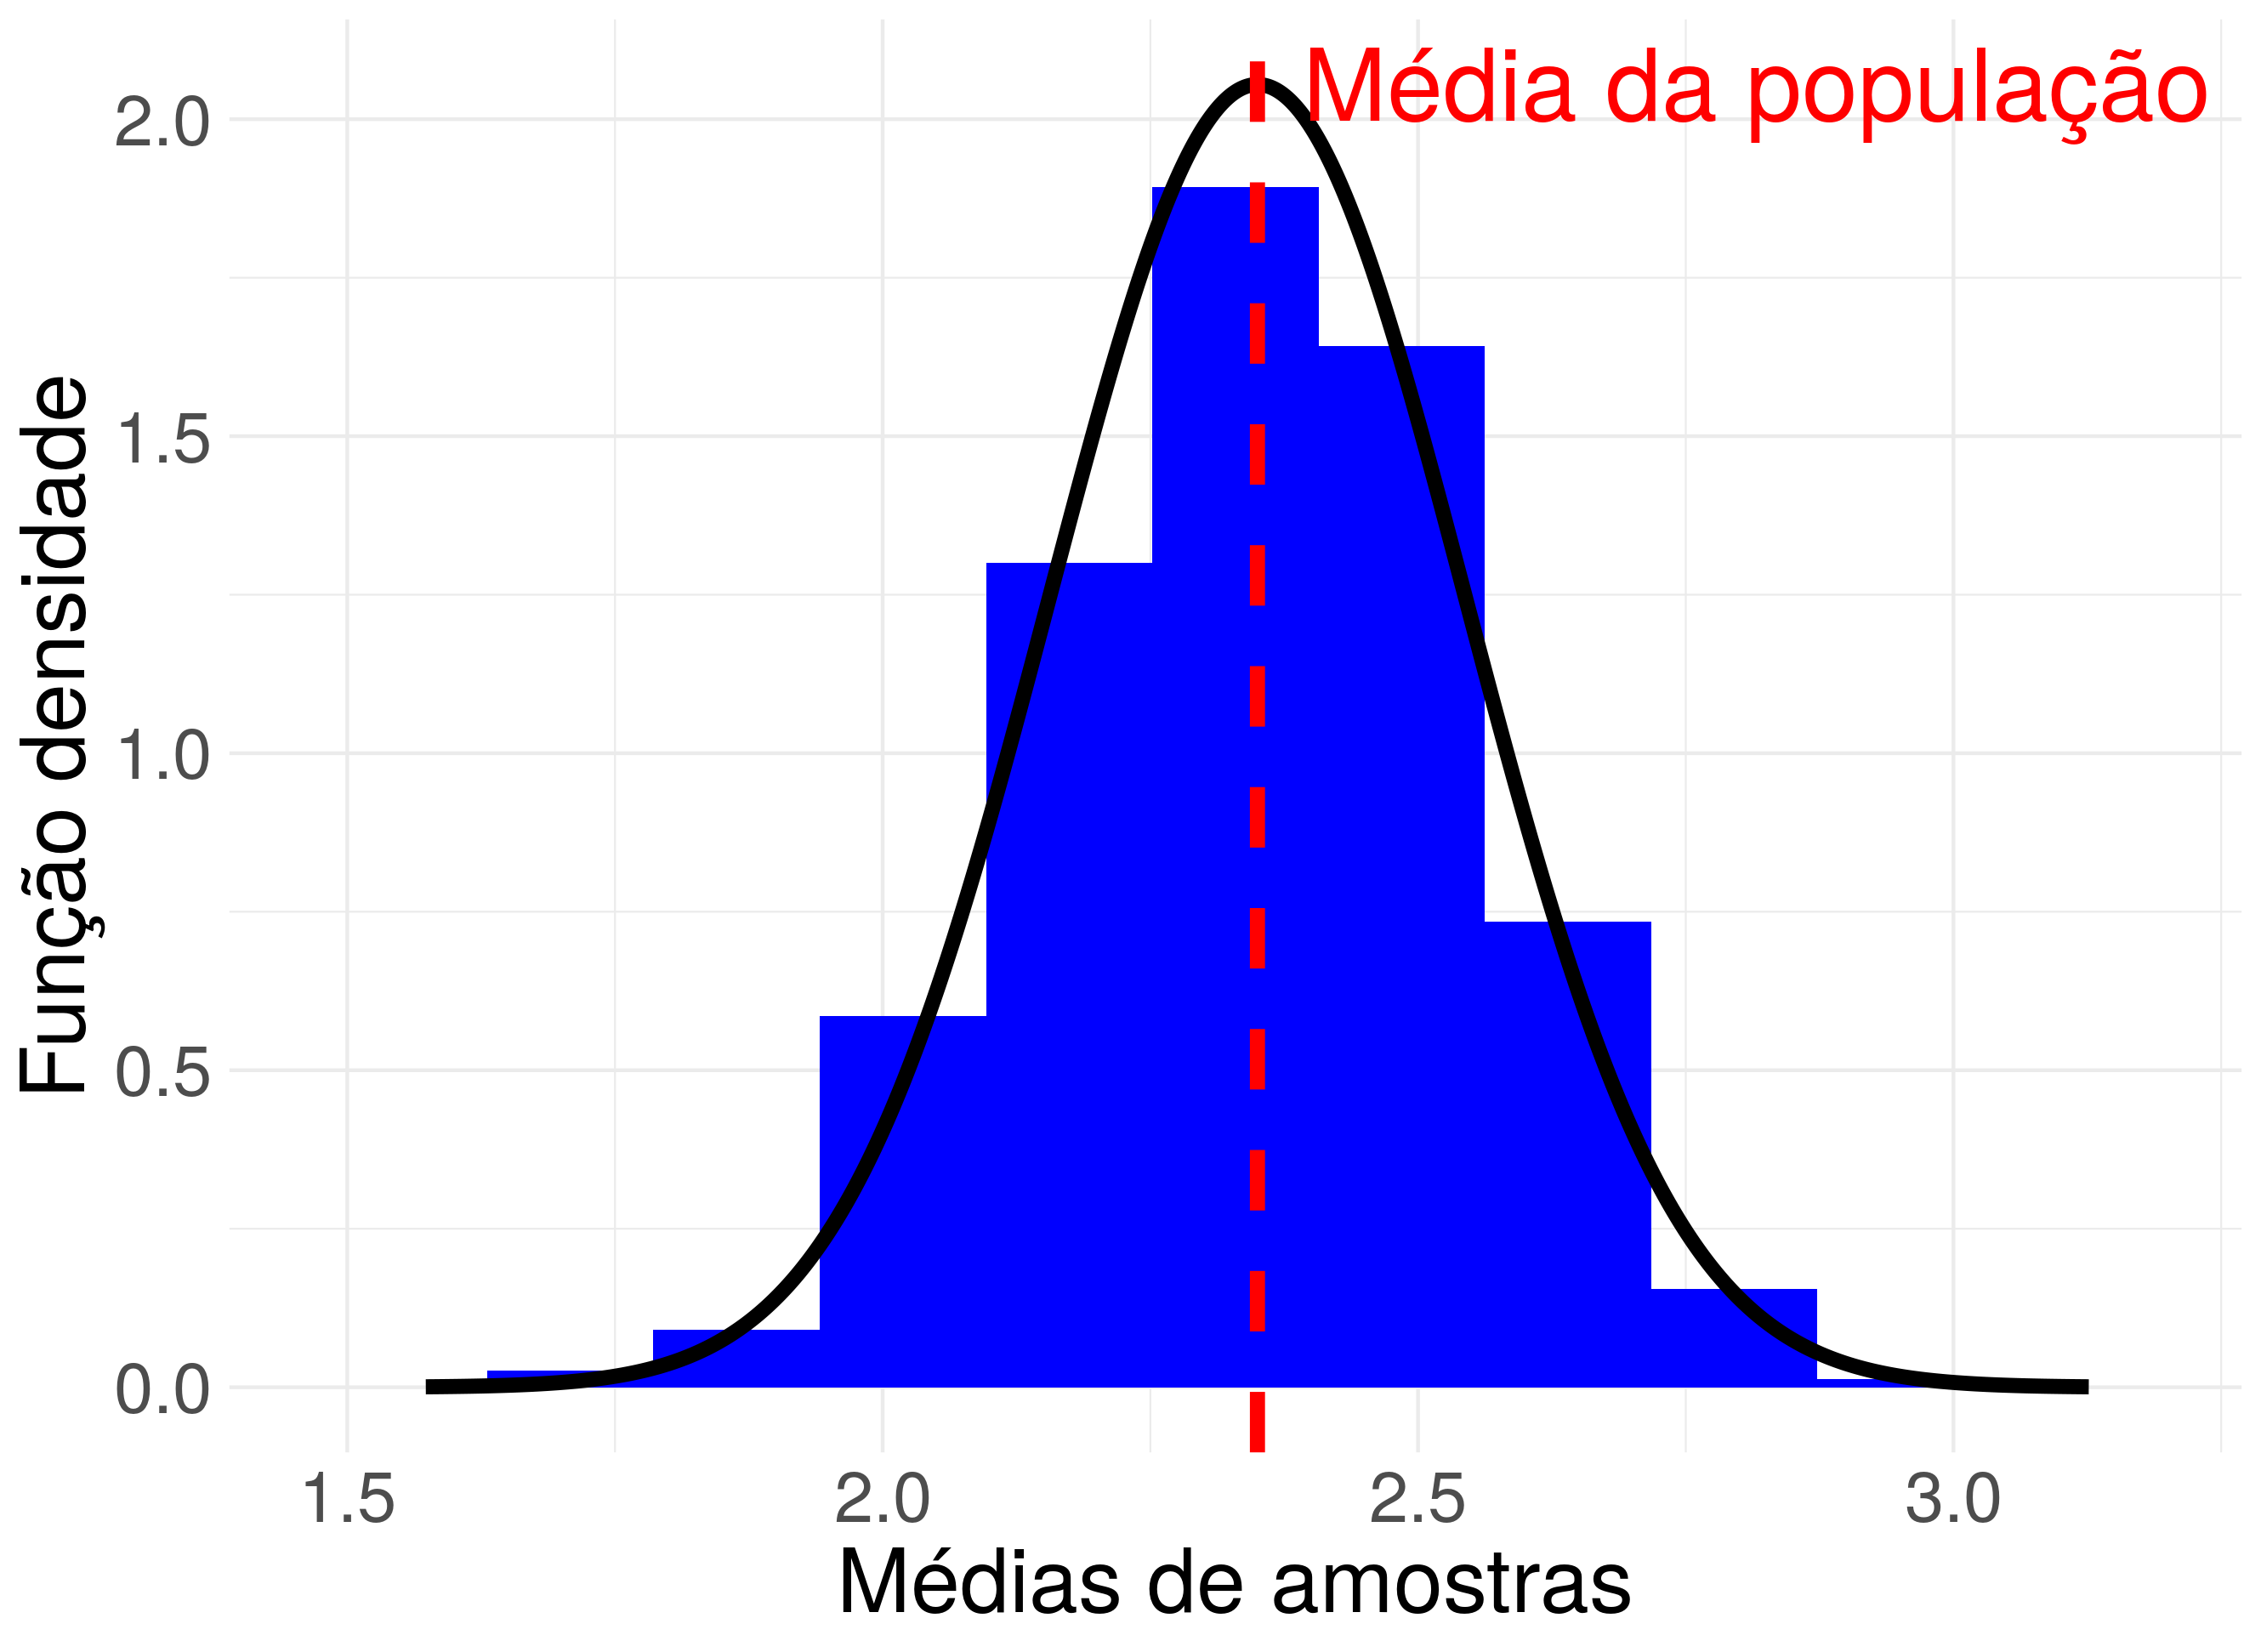
\includegraphics[width=.3\linewidth]{figure/amostras_discreta_75.png}}
	\caption{Médias das amostras: demonstração do teorema central do limite.}
	\label{fig:medias_disc}
\end{figure}

\end{frame}

\section{Teorema central do limite}

\begin{frame}{Teorema central do limite}
\begin{block}{Ideia}
 Para um tamanho de amostra suficientemente grande, a distribuição de $\bar{X}$ pode ser aproximada por uma distribuição normal, independente do modelo de probabilidade de $X_i$.
\end{block}
\vfill

\begin{block}{Teorema central do limite (amostras grandes)}
 Considere uma população com média $\mu$ e $\sigma^2$. Suponha que temos uma amostra $X_1, \dots, X_n$, então
 \begin{align*}
  \bar{X}  \sim Normal\left(\mu, \dfrac{\sigma^2}{n} \right).
 \end{align*}
\end{block}
\vfill

\begin{block}{Propriedade IMPORTANTE da distribuição Normal}
	\textcolor{red}{Se $x_1, \dots, x_m$ valores observados da variável aleatória $X \sim N(\mu, \sigma^2)$, então  $\bar{X} \sim Normal\left( \mu, \frac{\sigma^2}{n} \right)$.}
\end{block}
\end{frame}

\begin{frame}{Exemplo}
Em um estudo da altura de pacientes, escolhemos 10 pacientes. Sabemos que a altura dos pacientes tem distribuição normal com média $185cm$ e desvio padrão $40cm$. Qual a distribuição de $\bar{X}$?
Qual a probabilidade da altura média dos pacientes escolhidos ser maior que a média populacional?
\vfill

\textbf{Solução:}

\begin{itemize}
	\item $\bar{X} \sim Normal\left( 185, \dfrac{40}{10}  \right) $, ou seja, $\bar{X} \sim Normal\left( 185, 4 \right)$.
	\vfill
	
	\item
	\begin{align*}
	P(\bar{X} > 185) &= 1 - P(\bar{X} \leq 185)\\
	&= 1 - \Phi\left( \dfrac{185-185}{2} \right)\\
	&= 1 - \Phi(0) = 1 - 0,50 = 0,50
	\end{align*}
\end{itemize}


\end{frame}


\begin{frame}{Exemplo}
Considere uma variável aleatória discreta $X: \Omega \rightarrow \mathbb{R}$ que assume os valores $3, 6$, e $8$ com, respectivamente, probabilidades $0,5; 0,3$, e $0,2$. Uma amostra de 40 observações é 
sorteada, qual a probabilidade da média da amostra ser maior que 5?
\vfill

\textbf{Solução:} Primeiramente, note que
\begin{align*}
 \mu &= 0,5 \cdot 3 + 0,3 \cdot 6 + 0,2 \cdot 8 = 4,9,\\
 \sigma^2 &= 0,5 \cdot (3 - 4,9)^2 + 0,3 \cdot (6 - 4,9)^2 + 0,2 \cdot (8 - 4,9)^2 = 4,09.
\end{align*}

Usando o Teorema central do limite, temos que $\bar{X} \sim N\left(4,9; \dfrac{4,09}{40}\right)$ e 
\begin{align*}
 P(\bar{X} > 5) &=1-  P(\bar{X} \leq 5)\\
 &=1- \Phi \left( \dfrac{5 - 4,9}{\sqrt{ \frac{4,09}{40} }} \right)\\
 &= 1 - \Phi(0,32) = 1-0,6255=0,37.
\end{align*}

 
\end{frame}


\subsection{Distribuição Bernoulli}

\begin{frame}{Exemplo}
\begin{block}{Distribuição Bernoulli}
 Lembre que $\espe (X) = p$ e $\vari(X) = p(1-p)$.
\end{block}

\begin{block}{Exemplo}
 Suponha que a prevalência do vírus HIV na África Subsariana é $10\%$. Um médico selecionou 40 pacientes desta região. Qual a probabilidade de no máximo $20\%$ desses pacientes estarem infectados pelo vírus?
 \vfill
 
 \textbf{Solução:}  Pelo Teorema central do limite, temos que $\hat{p}  \sim N\left(0,1; \dfrac{0,1\cdot 0,9}{40}\right)$. Logo, temos que
 \begin{align*}
  P(\hat{p} < 0,2) &= \Phi \left(\dfrac{0,2 - 0,1}{ \sqrt{ \frac{0,1 \cdot 0,9}{40} } }\right) \\
  &= \Phi( 2,11)=0,9826
 \end{align*}

\end{block}

 
\end{frame}

\subsection{Distribuição poison}

\begin{frame}{Exemplo}

\begin{block}{Distribuição poison}
Lembre que $\espe(X) = \lambda$ e $\vari(X) = \lambda$.
\end{block}


\begin{block}{Exemplo}
 A emissão de partículas radioativas alfa de um isótopo em um minuto é modelada através de um distribuição poison com média 5. 
 Um físico analisar cinco amostras desse isótopo e observou o número de partículas alfa emitidas para  uma amostra com observações $x_1, x_2, x_3, x_4, x_5$. 
 Qual a probabilidade da média de partículas emitidas nessa amostra com cinco valores ser maior que seis?
 \vfill
 
 \textbf{Solução:} Pelo teorema central do limite, temos que $\bar{X} \sim N\left(\lambda, \dfrac{\lambda}{5}\right)$. Então
 
 \begin{align*}
  P(\bar{X} > 6) &= 1 - P(\bar{X} \leq 6)\\
  &= 1 - \Phi\left( \dfrac{6-5}{\sqrt{ \frac{5}{5} }} \right)\\
  &= 1 - \Phi( 1) = 1 - 0,8413 = 0,1587
 \end{align*}

\end{block}
\end{frame}

\subsection{Distribuição exponencial}

\begin{frame}{Exemplo}
 \begin{block}{Distribuição exponencial}
 Lembre que $\espe(X) = \frac{1}{\alpha}=\mu$ e $\vari(X) = \frac{1}{\alpha^2}=\mu^2$.
 \end{block}

 \begin{block}{Exemplo}
 Uma indústria fabrica lâmpadas especiais que ficam em operação continuamente. A fabricante afirma que as lâmpadas duram em média 8000 horas. 
 Um órgão de controle teste 10 lâmpadas. Assumindo que o fabricante diz a verdade, qual a probabilidade do órgão regulador obter uma média de no máximo 7000 horas para a amostra?
 \vfill
 
 \textbf{Solução:} Pelo teorema do limite central, temos que $\bar{X} \sim N\left( \mu; \dfrac{\mu^2}{ n} \right)$. Então,
 \begin{align*}
  P(\bar{X} < 7000) &= \Phi\left( \dfrac{7000 - \mu}{ \sqrt{\dfrac{\mu^2}{n}}}  \right) = \Phi \left( \dfrac{7000 - 8000}{ \sqrt{\dfrac{8000^2}{10}} } \right)\\
  &= \Phi( -0,4) \\
  &= 0,3446.
 \end{align*}

 \end{block}
\end{frame}



% \subsection{Modelo Gamma}


%
%\section{Exercícios em sala de aula}
%
%\begin{frame}{Exercícios em sala de aula}
%\begin{enumerate}[1.]
% \item Sendo $X \sim U[0,4]$, determine:
% \begin{enumerate}
%  \item $P(0 < X < 2)$;
%  \item $P(X < 2)$;
%  \item $P(1 < X < 4)$;
%  \item $P(X > 3)$;
%  \item $P(X < 2 \mid X > 1)$.
% \end{enumerate}
% 
% \item Seja $X \sim Exp(0,1)$, calcule
% \begin{enumerate}[a)]
%  \item $P(X\leq 5)$;
%  \item $P(4 < X< 6)$;
%  \item $P(2 \leq X < 5)$;
%  \item $P(X \leq \mid X > 2)$;
%  \item Qual o valor de $b$ tal que $P(X < b)=0,5$.
% \end{enumerate}
% 
% \item Para $X \sim N(90,100)$, obtenha
% \begin{enumerate}[a)]
%  \item $P(X \leq 115)$;
%  \item $P(X \geq 80)$;
%  \item $P(X \leq 75)$;
%  \item $P(85 \leq X \leq 110)$;
%  \item $P(\lvert X - 90 \rvert \leq 10)$;
%  \item O valor de $a$ tal que $P(90-a \leq X \leq 90+a)=0,95$.
% \end{enumerate}
%\end{enumerate}
%
%\end{frame}
%
%\begin{frame}{Exercícios em sala}
%\begin{enumerate}[1.]
% \item Uma clínica de emagracimento recebe pacientes adultos com peso seguindo uma distribuição Normal com média $130kg$ e desvio padrão $20kg$. Para efeito de determinar o tratamento mais adequado, os $25\%$ pacientes de menor peso são classificados de ``magros'', enquanto os $25\%$ de maior peso de ``obesos''. Determine os valores que delimitam cada uma dessas classificações.
% \item Dois amisgos planejam um encontro entre 20 e 21 horas. Um deles é pontual e pretende chegar às 20h30min e esperar exatos 15 minutos. O outro é mais imprevísivel e poderá chegar em qualquer momento do intervalo inicialmente previsto, saindo imediatamente se não encontrar o amigo. Qual é a probabilidade deles se encontrarem? Qual é a probabilidade deles não se encontrarem por um lapso de tempo de no máximo 5 minutos?
% \item O tempo necessário para eliminar o perigo de contaminação de um certo pesticida após sua aplicação em um pomar, é uma variável aleatória Exponencial de parâmetro 2 (em anos). Com probabilidade $99,9\%$, qual o tempo necessário para o consumo seguro após a aplicação do pesticida? Calcule a probabilidade de uma fruta desse pomar, escolhida ao acaso, não estar mais contaminada após um ano da pulverização.
%\end{enumerate}
%
% 
%\end{frame}


% \section{Estimação pontual dos parâmetros em modelos de probabilidade}
% 
% \begin{frame}
% \begin{block}{Objetivo}
%  Encontrar o valor do parâmetros dos modelos de probabilidade usando um amostra.
% \end{block}
% 
% Seja $x_1, \dots, x_n$ um amostra aleatória simples da variável quantitativa, então
% 
% {\footnotesize
% \begin{table}[ht]
%  \begin{tabular}{l|ccc}
%   \toprule[0.05cm]
%   Amostra & distribuição & Parâmetros & Estimador \\
%   \midrule[0.05cm]
%   $x_1, \dots, x_n$ & $Bernoulli(p)$ & $p$ & $\hat{p} = \dfrac{x_1 +  \cdots + x_n}{n}$\\
%   $x_1, \dots, x_n$ & $Poison(\lambda)$ & $\lambda$ & $\hat{\lambda} = \dfrac{x_1 + \cdots + x_n}{n}$\\
%   $x_1, \dots, x_n$ & $Exp(\alpha)$ & $\alpha$ & $\hat{\alpha} = \dfrac{1}{ \dfrac{x_1 + \cdots + x_n}{n}  }$\\
%   $x_1, \dots, x_n$ & $Normal(\mu, \sigma^2)$ & $\mu, \sigma^2$ & $\hat{\mu} = \dfrac{x_1 + \cdots + x_n}{n}$; $\sigma^2 = \dfrac{(x_1-\hat\mu)^2 + \cdots + (x_n-\hat\mu)^2}{n}$\\
%   \bottomrule[0.05cm]
%  \end{tabular}
% \end{table}
% }
% 
% \end{frame}
% 
% \begin{frame}{Exemplo}
%   Um pesquisador com interesse em estudar o tempo de vida de uma certa moléstia e coletou uma amostra com 15 pacientes conforme tabela~\ref{tab:pacientes}.
%   \begin{table}[ht]
%     \centering
%     \caption{}
%     \label{tab:pacientes}
%     \begin{tabular}{|ccccc|}
%       \hline
%     53 & 2 & 768 & 218 & 150 \\ 
%       63 & 55 & 151 & 27 & 48 \\ 
%       97 & 3 & 115 & 54 & 11 \\ 
%       \hline
%     \end{tabular}
%     \end{table}
%   Qual a probabilidade de um paciente sobreviver mais de 45 dias?
%   
%   \textbf{Solução:}
%   Note que $X \sim Exp(\alpha)$ e $\hat{\alpha} = \dfrac{1}{\frac{x_1 + \cdots + x_2}{n}}  = \dfrac{1}{121} = 0,008$.
%   \begin{align*}
%    P(45 < X) = \exp(-0,008 \cdot 45) = 0,7.
%   \end{align*}
% 
% \end{frame}


\end{document}